% !Mode:: "TeX:UTF-8" 

\BiChapter{跨项目克隆代码一致性维护需求预测研究}
{Cross-Project Clone Consistency-Requirement Prediction}

\BiSection{引言}
{Introduction}

由于日益增长的软件开发需求,复用既有代码作为一种常见的开发手段会引入大量克隆代码。随软件系统演化的过程中,克隆代码的一致性变化不仅会引发额外的维护代价,甚至可能会导致克隆一致性违背缺陷。因此,本文第3章和第4章在克隆代码创建和变化时,预测克隆代码的一致性维护需求。但是,第3章和第4章的方法无法应用于软件开发初期阶段的系统中。因为其未经过充分的演化,缺少克隆创建、变化实例训练机器学习模型。为解决此问题,本章在第3章和第4章研究的基础上,对跨项目的克隆代码一致性维护需求预测问题进行研究,可以在软件开发初期,帮助避免克隆额外维护代价和一致性违背缺陷。

鉴于此,针对软件开发初期项目缺乏训练数据的问题,本章研究了跨项目的克隆代码的一致性维护需求预测。首先,在第3章和第4章的研究的基础上,统一了克隆代码创建、变化的一致性维护需求定义。然后,将不同的软件系统划分为测试集和训练集,使用机器学习方法在训练系统上训练机器学习模型,在测试系统上验证跨项目模型的预测能力。在四个开源软件系统上进行了跨项目实证研究,实验结果表明:跨项目的克隆一致性维护需求预测,可以应用于软件开发初期时的预测中。同时,跨项目预测的效果依赖于具体的系统以及训练数据的规模。最后,结合软件开发过程,基于eclipse设计并实现了克隆代码一致性维护需求预测插件。所实现的克隆一致性维护需求预测插件,可以帮助程序人员边开发、边维护克隆代码,从而帮助提高软件质量和可维护性。

\BiSection{跨项目克隆一致性维护问题}
{The Problem for Cross-Project Clone Consistency Maintenance}

\BiSubsection{问题的提出}
{Problem in this Chapter}

%在软件开发过程中,复用既有代码已经成为一种常见的软件开发手段。但是,也会向软件系统中引入大量的克隆代码。引入系统中的克隆代码随着系统进行演化,在演化过程中会被软件开发员修改,并可能导致克隆代码的一致性变化。克隆一致性变化问题是影响软件质量和可维护性的重要原因:一致性变化会导致额外的一致性维护代价,而遗忘一致性变化,更会导致克隆一致性违背缺陷。

为了解决克隆代码的一致性维护问题,本文的第3章和第4章分别在克隆代码创建时和变化时,预测克隆代码的一致性维护需求。但是,上述方法仅仅适用于软件经过若干版本演化,系统具有充足的克隆创建和变化实例数据的情况。

然而,在软件开发初期阶段,尤其是软件开发的第一个版本时,系统刚开始进行演化,一般不具有充足的历史演化数据(第一个版本甚至没有相关数据),从而无法有效地预测克隆代码的一致性维护需求。因此,这启发了本章对跨项目的克隆代码的一致性维护需求的研究。值得注意是,在现有的研究中,还尚未有人研究跨项目的克隆代码一致性维护问题,本章的研究将对跨项目的克隆一致性维护研究提供一个新的解决思路和方案。此外,本文第3章和第4章中仅给出了克隆一致性维护需求的预测方法,并没有具体结合软件开发过程,帮助程序开发人员进行克隆代码的一致性维护需求的预测。

%%%目前的研究依然存在以下两点不足之处:
%%%
%%%(1)在软件开发的初始阶段,由于缺乏项目自身训练数据不足的问题,本章对克隆代码的一致性维护需求进行跨项目的预测研究。对于某一软件系统,将使用其它项目的数据训练预测模型,并预测其一致性维护需求。
%%%
%%%(2)缺乏

综上,在软件系统开发的早期阶段,系统没有经过充分的演化,缺乏相应的训练数据,无法对其进行一致性维护需求预测,因而无法避免克隆代码的额外维护代价和一致性违背缺陷。因此,如何使用跨项目的数据(其它项目数据)对克隆代码进行一致性维护需求预测是一个值得研究的问题。同时,结合软件开发过程,对克隆代码进行一致性维护需求预测,可以帮助开发人员实现边开发、边维护克隆代码,提高软件质量和可维护性。

\BiSubsection{本文的解决思路}
{The Proposed Method}

为解决本章所提出的跨项目的克隆代码一致性需求维护预测问题,本节给出本章方法的框架。跨项目克隆代码一致性需求预测框架如图~\ref{framework5}~所示。跨项目的克隆一致性维护需求预测方法可以划分为三个阶段,分别为训练数据收集阶段、测试数据收集阶段和跨项目预测阶段。收集阶段旨在收集训练系统和测试系统中全部的克隆实例(包括创建实例和变化实例),并将训练系统的数据集用于机器学习模型的构建,测试系统的数据用于测试跨项目预测的效果。在预测阶段,使用训练系统数据所构建的机器学习模型预测测试系统的克隆代码一致性维护需求。其中,在表示所收集到的克隆实例时,也会提取相应的属性值描述所提取的克隆实例,所提取的属性值与第3章和第4章中的相同。

\begin{figure}[htbp]
\centering
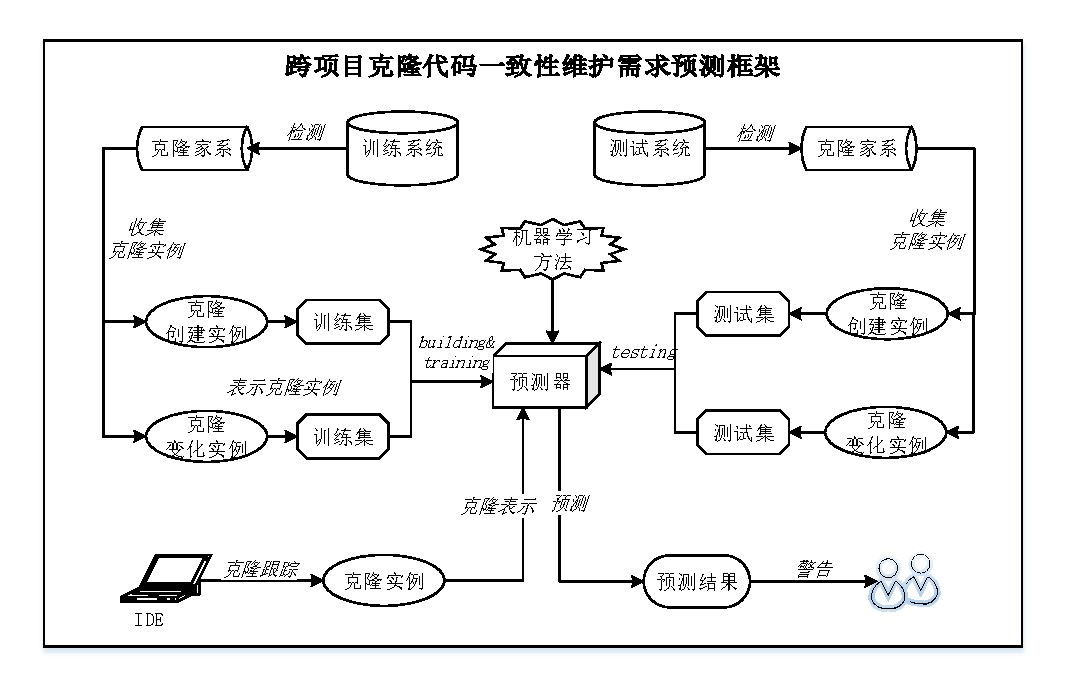
\includegraphics[width = 0.8\textwidth]{framework5.pdf}
\bicaption[framework5]{}{跨项目克隆代码一致性维护需求预测框架}
{Fig.$\!$}{The framework for clone cross-project consistency prediction}
\vspace{-1em}
\end{figure}

为了收集不同系统中的克隆代码创建和变化实例,同样通过构建系统的克隆家系来完成收集工作。使用NiCad来检测软件版本中的所有克隆,并通过在相邻版本的克隆组之间进行映射来构建克隆家系,用于收集克隆实例。然后,通过提取属性值表示克隆创建和变化实例,分别提取代码属性和上下文属性表示克隆创建实例,提取代码属性、上下文属性和历史属性表示克隆变化实例。最后,使用收集到的训练系统的克隆实例训练机器学习模型,并使用其预测测试系统的克隆代码一致性维护需求。

与第3章和第4章相似,每一个克隆实例也有两种不同的预测结果,即满足一致性维护需求和不满足维护需求。
对于满足一致性维护需求实例来说,其在将来的演化中可能会引发一致性变化,程序开发人员需要采取相应的操作。例如,拒绝克隆创建实例或者检查克隆变化实例的一致性。对于不满足一致性维护需求实例来说,其在将来的演化中不会引发一致性变化,程序开发人员不需要需要采取相应的操作,可以放心自由的接受新创建的克隆实例和修改克隆代码。

本章在第3章和第4章的研究基础上,在进行跨项目的克隆一致性维护需求预测时,将同时预测克隆代码创建时和变化时的跨项目一致性维护需求,将重点分析和讨论如下问题:

%%(1)如何描述和定义克隆代码的一致性变化和一致性维护需求?
%%(2)如何收集和系统中跨项目的数据
%%(3)如何结合软件开发过程,。。。同时,还可以划分为三个子问题

(1)在软件开发初期阶段,在项目自身训练数据不充分的情况下,能否使用其它系统的数据训练模型,并对该系统进行克隆一致性需求预测?

(2)在进行跨项目的克隆一致性维护需求预测时,训练数据的规模将如何影响跨项目的预测效果?%应该如何选择跨项目预测的数据集,以达到更好的预测效果?

(3)在进行跨项目的克隆一致性维护需求预测时,应该预测哪一类别的克隆代码实例,是否对两种不同类别的实例都具有相一致的预测效果?

\BiSection{克隆一致性维护需求的定义}
{The Definitions for Clone Consistency-Requirement}

在克隆代码的整个演化周期中,克隆片段可能会被开发人员修改,从而导致克隆代码的一致性变化。在本文的第3章和第4章分别提供了两种不同形式的克隆代码一致性变化定义,从而适应于不同时间的克隆一致性维护需求预测中。为了进一步研究跨项目的一致性预测问题,本节统一了第3章和第4章的定义,以应用于跨项目的克隆代码一致性维护需求预测中。因此,克隆代码的一致性变化如下:

\begin{definition}[克隆一致性变化]  
\label{def-change}
给定两个克隆代码片段 $CF_1$和 $CF_2$,且它们被分别地修改为$CF'_1$和$CF'_2$。 如果对于一个非常小的阈值$\tau$,如果克隆代码$CF_1$和$CF_2$的变化满足以下条件,称此变化为一致性变化(Consistent Change) , 
\[
\begin{array}[t]{crl}
 \mathit{textSim}(CF_i, CF'_i) < 1 & \forall i \in \{1,2\} &(1) \\
 \multicolumn{2}{c}{| ~\mathit{textSim}(CF_1,CF'_1)  ~-~ \mathit{textSim}(CF_2,CF'_2) ~| ~< ~ \tau}  & (2)
\end{array}
\]
如果克隆代码变化仅满足条件1,将其称为Type-1一致性变化(Type-1 Consistent Change);如果克隆变化同时满足条件1和条件2,将其称为Type-2一致性变化(Type-2 Consistent Change)。
\end{definition}

定义中克隆代码$ CF_1 $和$ CF_2 $的变化情况由相似性度量$ \mathit {textSim} $进行定义,$textSim$与第3章和第4章计算方式相同。该定义中的两个约束条件共同定义了克隆代码的一致性变化,约束条件$1$确保了克隆代码片段同时被修改,约束条件$2$克隆代码片段发生了一致性的变化,由阈值$\tau$指定。

其中,Type-1一致性变化是克隆创建一致性变化,Type-2一致性变化是克隆变化的一致性变化。这两种不同的一致性变化,将分别应用于两种不同时间的克隆一致性预测中。在克隆代码创建时,目标是避免新创建的克隆代码在其未来演化过程中的一致性变化,及其所导致额外的维护代价。所以,只要两个克隆片段同时变化,即认为会导致额外维护代价。因此,在克隆代码创建时使用使用Type-1一致性变化进行预测。在克隆代码变化时,目的是避免克隆变化可能导致的未来演化中的一致性变化,及其因此所引发的克隆一致性违背缺陷。所以, 不仅要求两个克隆代码片段同时变化,还需要发生相似的变化,否则将会引入克隆一致性违背缺陷,因此,在克隆代码变化时使用使用Type-2一致性变化进行预测。

在克隆演化过程中,克隆片段是以克隆组的形式出现在软件系统中。克隆代码的变化情况必然会导致克隆组的变化,而克隆组的变化使用克隆演化模式进行描述,即一致性变化模式。现给出演化过程中克隆组的一致性变化模式定义,如下所示:

\begin{definition}[克隆一致性变化模式] 
\label{def-pattern}
在软件版本 $j+1$中存在一个克隆组$CG'$ ,假设克隆组内至少存在两个克隆代码片段$CF'_1$ 和 $CF'_2$可以与映射到上一版本$j$的克隆组$CG$中,且 $CG$中与之对应的克隆代码片段的 $(CF_1,CF_2)$被修改为$(CF'_1,CF'_2)$。如果克隆片段之间的变化 $(CF_1,CF_2)$变化至$(CF'_1,CF'_2)$满足克隆片段的“Type-1或者Type-2一致性变化”(Type-1 or Type-2 Consistent Change),则称克隆组$CG'$具有Type-1或者Type-2一致性变化模式(Type-1 or  Type-2 Consistent Change Pattern)。
\end{definition}

回顾本章地研究内容是要在两种不同的时刻,跨项目的预测克隆代码的一致性维护需求,结合第3章和第4章的克隆实例的定义,这里将统克隆创建实例和克隆变化实例统一为克隆实例,如下所示:

\begin{definition}[克隆实例] 
\label{def-instance}
将克隆创建实例和克隆变化实例统称为克隆实例。在一个克隆家系$CG$中,克隆家系的根节点为克隆创建实例,并且发生变化的克隆组为克隆变化实例。
\end{definition}

克隆实例在演化过程中可能会发生一致性变化模式,如果不能确保克隆的一致性,将会导致导致额外的维护代价和一致性违背缺陷。对于克隆创建实例,Type-1一致性变化可能会导致额外的克隆维护代价。对于克隆变化实例,Type-2一致性变化可能会导致克隆一致性违背缺陷。因此,需要在不同时间预测克隆实例的一致性维护需求,以避免额外的克隆维护代价和一致性违背缺陷。本章结合第3章和第4章的克隆代码一致性维护需求的定义,将克隆创建和变化的一致性维护需求统一为克隆一致性维护需求定义,如下所示:

\begin{definition}[克隆一致性维护需求] 
 \label{def-requirement}
给定版本 $j$中一个克隆实例,$CG$满足克隆一致性维护需求(Consistency-Requirement),如果在版本$k$中存在一个克隆实例 $CG'$($k>j$)满足以下条件: (1) 在$CG'$中至少存在两个克隆片段在其克隆家系$CGE$中可以映射到克隆实例 $CG$中, (2) $CG'$ 具有“Type-1或者Type-2一致性变化模式”(Type-1 or Type-2 Consistent Change Pattern)。反之,假如克隆实例$CG$ 不满足克隆一致性维护需求条件,称该克隆实例不需要一致性维护(Consistency-Requirement Free,或者Consistency-Free,或者Free)。
\end{definition}

最终,克隆一致性维护需求预测可以转化为以下问题:给定一个克隆实例,克隆创建实例或者克隆变化实例,判断该克隆实例是否满足克隆一致性维护需求。

\BiSection{跨项目数据集的获取}
{Collecting the Dataset for Cross-Project Prediction}

在跨项目的预测中,使用其它系统的数据训练机器学习模型,并预测另外系统的一致性维护需求。因此,需要构建跨项目的数据集,将从训练系统中提取克隆实例作为训练集,从测试系统中提取克隆实例作为测试集。

对于某一个软件系统来讲,通过收集和表示该系统中的克隆实例,可以生成其数据集。因此,生成实验所需的数据集,可以划分为两个部分:收集系统中的克隆实例和表示所收集到的克隆实例

\BiSubsection{跨项目数据来源}
{Data Sources for Cross-Project Prediction}

跨项目的数据由软件系统中的克隆实例组成,因此收集系统中的克隆实例,即可以完成收集跨项目的数据。通过构建系统的克隆家系,通过识别其中的克隆演化模式,可以从软件中收集所有的克隆实例。根据定义~\ref{def-instance}~,克隆家系$CGE$中的初始节点即是克隆创建实例,发生变化的克隆组是变化实例。通过构建和遍历克隆家系,可以收集克隆创建和变化实例。

首先,下载系统所有版本的源代码,通过映射所有相邻版本的克隆代码,构建系统中全部克隆家系。然后,通过对比相邻版本的克隆代码,识别克隆家系的克隆演化模式,尤其是克隆一致性变化模式(参考定义~\ref{def-evolutionpattern}~和\ref{def-pattern}~)。根据定义~\ref{def-instance}~通过遍历克隆家系的根节点,可收集系统中所有的克隆创建实例。在收集克隆创建实例后,还需确认该实例中的被复制和被粘贴代码(参见本文第3章收集克隆创建实例小节~\ref{lab-checkcopied}~)。根据定义~\ref{def-instance}通过识别克隆家系中的变化克隆组,便可以收集系统中的克隆变化实例。

根据定义~\ref{def-requirement}~,通过遍历克隆实例所在的克隆家系$CGE$的演化情况,标识克隆实例的一致性维护需求。如果克隆实例在其演化过程中发生了一致性变化模式(定义~\ref{def-pattern}~),则该实例满足一致性维护需求,否则不满足维护需求。

\BiSubsection{属性特征与数据集生成}
{The Attributes and Generation for Data Set}

本文收集到的数据是系统中的克隆实例,因此同样提取相应的属性值表示克隆代码实例。将提取代码、上下文两组属性代表克隆创建实例,提取代码属性、上下文属性和演化属性代表克隆变化实例。其中,代码属性和上下文属性相似,但从不同的角度表示克隆创建实例和变化实例。克隆创建实例中的属性,表示了创建时克隆代码的特征;克隆变化实例中的属性,表示了发生变化的克隆组的特征。

对于克隆创建实例,即被复制和粘贴克隆代码,使用不同的属性进行描述。使用代码属性用于表示被复制的克隆的特征,包括:克隆代码粒度、Halstead属性、结构属性、参数访问数量、总函数调用次数、本地函数调用次数、库函数调用次数、其它调用次数。使用上下文属性用于表示被粘贴的克隆代码的特征,包括:代码相似度、局部克隆标识、文件名相似度、文件名相似度标识、方法名相似度、总参数名相似度、最大参数名相似度、总参数类型相似度、块信息标识。属性具体信息可以参考本文第3章相关属性值部分(第~\ref{lab-creatingattribute}~节克隆创建实例表示)。

对于克隆变化实例,从克隆组的角度重新提取了代码属性和上下文属性,并从演化的角度新增演化属性。代码属性从代码自身的角度,描述了克隆变化实例中克隆代码特征,包括克隆粒度、代码行平均、Halstead属性平均、结构属性平均、总函数调用次数平均、本地函数调用次数平均、库函数调用次数平均、其它调用次数平均。上下文属性描述了克隆变化实例所在克隆组的克隆关系特征,包括代码相似度平均、文件名相似度平均、文件名相似度变量、方法名相似度平均、总参数名相似度平均、最大参数名相似度平均、总参数类型相似度平均、块信息标识。历史属性描述了克隆变化实例所在克隆组在克隆变化发生前的历史演化特征,包括变化实例寿命、历史演化模式统计、当前演化模式、历史变化统计。同时,还提供了克隆变化实例的变化属性。
属性具体信息可以参考本文第4章相关属性值部分(第~\ref{lab-changingattribute}~节克隆变化实例表示)。

数据集生成算法如~\ref{alg-collection}~所示。算法中第1-5行是为克隆代码生成CRD,并使用CRD映射相邻版本的克隆代码,并根据克隆演化模式定义,识别克隆演化模式。第6行是生成系统的克隆家系。第7-10行,分别是收集克隆实例,并标记其一致性维护需求。第11行是初始化数据集。第12-15行是提取相应的属性值表示克隆实例,并且生成数据集。在表示克隆实例时,算法将消耗大量的时间,其时间复杂度为$O(m*n)$,其中m为克隆变化实例的数量。因此,该算法的时间复杂度为$O(m*n)$。

\begin{minipage}{0.8\textwidth}
\centering
\begin{algorithm}[H]
\AlgoBiCaption{数据集生成算法} {The algorithm for generating dataset}
\label{alg-collection}
\KwIn{All source code and code clones from $N$ versions}
\KwOut{The data set of software}
\For{$i$=1 to $N$}
{ 
 Generating CRD to represent each code clone{CFs}\;
 Mapping all the $CFs$ and $CGs$ between the adjacent versions {i} and {i+1}\;
 Identifying all clone evolution pattern in thus two versions according to Definition~\ref{def-evolutionpattern}~and~Definition~\ref{def-pattern}~\;
}
Generating all clone genealogies $CGEs$ with number $N\_cge$\;
\For{$i$=1 to $N\_cge$}
{ 
 Collecting the clone instance that both including clone-creating and changing instances from $CGE\_i$ according to Definition~\ref{def-instance}~\; 
 Labeling all consistency-requirement according to Definition~\ref{def-requirement}~;
}
Initializing all training data set $Creating\_Set$ and $Changing\_Set$for clone creating and changing instances\; 
\For{each clone instance} 
{ 
Generating all attributes for clone creating or changing instance\;
Appending all the attributes to the $Creating\_Set$\ or $Changing\_Set$\;
}
\Return {The data set of software\;}
\end{algorithm}
\end{minipage}

\BiSection{跨项目模型的构建与预测}
{Building the Cross-Project Models and Predicting}

使用收集到的训练系统的克隆实例训练机器学习模型,并预测测试系统的克隆代码的一致性维护需求。从而验证跨项目的克隆一致性需求的预测能力。值得注意的是,将对两种不同的时刻的克隆代码的一致性维护需求分别进行预测(即克隆创建时和克隆变化时),因此会训练两种不同的模型以适用于两个时刻。

对于所测试的软件系统,首先,通过收集训练系统中所有的克隆实例(创建实例和变化实例),并提取相应的属性,用于构建模型训练所需的数据集。然后,调用WEKA中的机器学习算法,分别构建克隆创建和变化的预测器,预测克隆代码的一致性维护需求。

跨项目克隆一致性维护需求预测算法如~\ref{alg-crossperdiction}~所示。算法的第1行为划分训练集和测试集。第2-3行是生成跨项目的数据集。第4行是使用训练集训练机器学习模型。第5行是使用训练的模型在测试集上验证跨项目预测的有效性。

\begin{minipage}{0.8\textwidth}
\centering
\begin{algorithm}[H]
\AlgoBiCaption{跨项目克隆一致性维护需求预测算法} {The algorithm for cross-project predicting clone consistency-requirement}
\label{alg-crossperdiction}
\KwIn{All the projects}
\KwOut{The predictive models}
Dividing the projects into training projects and testing project\;
Generating the $Training\_{Set}$ for training projects\;
Generating the $Testing\_{Set}$ for testing project\;
Calling WEKA to train the models applying training set $Training\_{Set}$\;
Employed this trained model to predict on the $Testing\_{Set}$\;
\Return {The predictive models\;}
\end{algorithm}
\end{minipage}

与第3章和第4章相似,根据定义~\ref{def-requirement}~,克隆实例会有两种不同的状态:需要一致性维护和不需要一致性维护。如下所示:

\begin{itemize}
\item 
需要一致性维护:
若克隆创建实例的预测结果为“需要”,软件开发人员需要谨慎的执行克隆创建操作。因为,该克隆创建实例,在未来演化的过程中可能会引发一致性变化,从而向系统中引入额外的维护代价。若克隆变化实例的预测结果为“需要”,软件开发人员需要检测克隆变化实例所在的克隆组的一致性问题,考虑一致地修改组内其它的克隆代码。因为该克隆变化实例,在未来演化的过程中可能会引发一致性变化,遗忘这种变化会向系统中引入缺陷,从而降低软件质量。
\item
不需要一致性维护:
若克隆创建实例的预测结果为“不需要”,软件开发人员可以自由的执行克隆创建操作,从而节约开发时间提高开发效率。因为该克隆创建实例,在未来演化的过程中不会引发一致性变化,也不会导致额外的维护代价。若克隆创建实例的预测结果为“不需要”,软件开发人员可以自由的修改克隆变化实例所在克隆组的克隆片段。因为,该克隆变化实例,在未来演化的过程中不会引发一致性变化,也不会导致一致性违背缺陷。
\end{itemize}

在使用已训练好的模型进行预测时,可以与软件开发过程相结合,将该模型嵌入到软件开发环境中,帮助程序开发人员实现边开发边预测克隆实例的一致性维护需求。首先,在软件开发环境中需监测和跟踪克隆代码,识别新产生的克隆实例(克隆创建实例和变化实例)。然后,根据上文描述的代码、上下文和演化属性,提取相应的特征表示相应的克隆实例。最后,使用训练好的预测器预测相应克隆实例的一致性维护需求,根据预测结果提醒程序开发人员采取进一步的操作。

\BiSection{实验结果与分析}
{Experimental Results and Analysis}

本节给出本章的实验结果与分析,使用五种不同的机器学习方法,对克隆代码创建时和变化时进行跨项目的一致性维护预测。首先简单介绍了实验所使用的实验系统和评估方法,然后详细给出每个实验的结果与分析。

\BiSubsection{实验设置}
{Experimental Methodology}

为了解决本章所提出的研究问题,本节选取和第3章和第4章相同的四个开源项目进行实验评估。四个实验系统的基本数据集如表~\ref{instancesta}~所示,分别包括克隆创建实例和克隆变化实例。从该表可以看出,系统中克隆创建实例的数据集的规模要大于克隆变化实例的数据集。克隆创建实例数据集规模为为633到3666个,克隆变化实例的数量范围在159到1040个,系统jEdit是克隆规模最小的系统。同时,表中第3和4列给出了不需要和需要一致性维护的克隆实例的数量和比例。


从表~\ref{instancesta}~中可以观察到两个现象。第一,软件系统中存在大量的克隆创建实例(三个项目中有上千的实例),同时大部分的克隆创建实例在其演化过程中不满足一致性维护要求(比例从59.8\%到88.47\%)。这表明克隆创建操作(即复制和粘贴操作)已经成为开发人员的常用技术,并且它们中的大多数在演化过程中不会在将来引入任何一致的变化,建议开发人员可以使用复制和粘贴操作节省开发时间。第二,在克隆变化实例中,三个系统中只有数百个变化实例,仅有jFreeChart中有1040变化实例。这表明相对于克隆代码在演化过程中不会频繁地发生变化,但也有相当数量的变化。值得注意的,这些变化中需要一致性维护的变化实例比例占相当大的一部分,其比例为33\%到74 \%。克隆代码的一致性变化更容易引发一致性变化,从而导致增加克隆代码一致性违背缺陷的风险,因此开发人员在软件开发过程中应该更加注意软件开发过程中的克隆变化。

\begin{table}[htbp]
\bicaption[instancesta]{}{实验系统基本数据集信息统计}
{Table$\!$}{The statistics for clone instances in four projects}
\vspace{0.5em}
\centering
\wuhao
\begin{tabular}{ccccc}
\toprule[1.5pt]
~\multirow{2}{*}{类型}&\multirow{2}{*}{系统}&{不需要}&{需要}&\multirow{2}{*}{总数}\\
~&~&{一致性维护}&{一致性维护}&~\\
\midrule[1pt]
\multirow{4}{*}{克隆创建实例}
&ArgoUML&	2574(77.07\%)&	766(22.93\%)&	3340\\
&jEdit&560(88.47\%)&	73(11.53\%)&	633\\
&jFreeChart&	2013(59.80\%)&	1353(40.20\%)&	3366\\
&Tuxguitar&	1016(71.10\%)&	413(28.90\%)&	1429\\
\hline
\multirow{4}{*}{克隆变化实例}
&ArgoUML&288(67.45\%)&139(32.55\%)&427\\
&jEdit&78(49.06\%)&81(50.94\%)&159\\
&jFreeChart&452(43.46\%)&588(56.54\%)&1040\\
&Tuxguitar&91(25.71\%)&263(74.29\%)&354\\
\bottomrule[1.5pt]
\end{tabular}
\end{table}

同时,在跨项目预测是,本文将使用三个系统的数据作为训练集,使用第四个系统作为测试集。因此,给出在进行跨项目预测时训练集规模的大小,如表~\ref{crosssta}~所示。表中使用(To Project)表示被测试的系统为“Project”,并使用除“Project”系统外其它的系统作为训练集。从表中发现克隆创建的训练集规模要远远大于克隆变化的训练集规模,其中克隆创建的训练集规模为5402-8135,克隆变化的训练集规模为940-1821。由于系统之家的差异,不同训练集的规模大小也不相同。

\begin{table}[htbp]
\bicaption[crosssta]{}{跨项目数据集信息统计}
{Table$\!$}{The statistics for cross-project data set}
\vspace{0.5em}
\centering
\wuhao
\begin{tabular}{ccccc}
\toprule[1.5pt]
~\multirow{2}{*}{类型}&\multirow{2}{*}{测试系统}&\multicolumn{3}{c}{训练集规模}\\
\cline{3-5}
~&~&{不需要维护}&{需要维护}&{总数}~\\
\midrule[1pt]
\multirow{4}{*}{克隆创建时}
&(To ArgoUML)&3589(66.12\%)&1839(33.88\%)&5428\\
&(To jEdit)&5603(68.88\%)&2532(31.12\%)&8135\\
&(To jFreeChart)&4150(76.82\%)&1252(23.18\%)&5402\\
&(To Tuxguitar)&	5147(70.13\%)&2192(29.87\%)&	7339\\
\hline
\multirow{4}{*}{克隆变化时}
&(To ArgoUML)&621(39.99\%)&932(60.01\%)&1553\\
&(To jEdit)&831(45.63\%)&990(54.37\%)&1821\\
&(To jFreeChart)&457(48.62\%)&483(51.38\%)&940\\
&(To Tuxguitar)&	818(50.31\%)&808(49.69\%)&1626\\
\bottomrule[1.5pt]
\end{tabular}
\end{table}

为解决跨项目克隆代码一致性预测问题,本章将研究问题划分为三个子研究问题。因此本节也将从三个不同的角度进行实验,并同时回答本文提出的三个子研究问题。三个实验如下:
\begin{itemize}
\item
跨项目的预测效果实验:将回答第一个子研究问题,使用不同的机器学习模型进行跨项目克隆一致性预测,以验证是否能使用跨项目的数据进行跨项目一致性维护需求预测。
\item
跨项目预测的数据集规模实验:将回答第二个子研究问题,使用不同的数据集训练机器学习模型,并在同一系统上测试跨项目预测模型的预测能力,从而确定训练集规模对跨项目模型预测能力的影响。
\item
跨项目预测的类别选择实验:将回答第三个子研究问题,将探讨在进行跨项目预测时,不同类别克隆实例的一致性预测的效果。实验将使用贝叶斯网络预测不同类别的克隆实例。
\end{itemize}

\BiSubsection{跨项目有效性验证实验}
{The Effectiveness Experiments for Cross-Project Prediction}

本节将回答本章提出的第一个研究问题:在软件开发初期阶段,在项目自身训练数据不充分的情况下,能否使用其它系统的数据训练模型,并对该系统进行克隆一致性维护需求预测?

在五种机器学习方法上进行了跨项目的预测,并使用同本文第3章和第4章相同的指标评估预测效果,即采用平均精确率(Average Precision)、平均召回率(Average Recall)和平均F值(Average F-measure)进行评价(见本文第~\ref{ref-creatingmetrics}~节和第~\ref{ref-changingmetrics}~节)。

\BiSubsubsection{克隆创建时的实验结果}
{The Results for Clone Creating Instances}

对克隆代码创建实例,使用不同的机器学习方法进行跨项目预测,实验结果如~\ref{creatingcrossmethodaverage}~所示。在表中,对于SVM的实验结果使用{*}进行标记表。原因在于:在使用SVM方法进行跨项目预测时,不具备相对应的预测能力,其会将所有的测试数据划分到同一个类别中(规模比较大的类中)。

从表\ref{creatingcrossmethodaverage}~中可以看出,除了SVM方法外,其它的四种机器学习方法,对不同的项目均具有不错的预测效果,并且彼此之间也不存在显著的差异。ArgoUML系统的预测结果较好,其平均F值介于65.3\%-66.7\%之间。对jEdit系统的预测效果最好,为76.2\%-82.6\%,jFreeChart最差,也达到了48.9\%-60.9\%。对于Tuxguitar来说,预测效果也较好,F值为60.3\%-68.3\%。

尽管如此,不同的机器学习方法在不同的跨项目的预测中,其预测能力不是完全一致。对系统ArgoUML和系统Tuxguitar来说,决策树具有最好的预测效果,其F值分别为66.7\%和68.3\%。贝叶斯网络对jEdit系统具有最好的预测效果,F值为82.6\%。而KNN方法对于系统jFreeChart具有最好的预测效果,F值为60.9\%。

因此,针对不同的系统,不推荐程序开发人员选用SVM的方法;但可以使用其它的机器学习方法进行跨项目的一致性维护需求预测;针对不同的软件系统,程序开发人员可以根据预测结果选择最合适的机器学习方法。

\begin{table}[htbp]
\bicaption[creatingcrossmethodaverage]{}{克隆创建时跨项目预测效果}
{Table$\!$}{The effectiveness for cross-project prediction at creating time}
\vspace{0.5em}
\centering
\wuhao
\begin{tabular}{cccccc}
\toprule[1.5pt]
{指标}&{方法}&{To ArgoUML}&{To jEdit}&{To jFreechart}&{To  Tuxguitar}\\
\midrule[1pt]
\multirow{5}{*}{平均Precision}
&BayesNet&	0.638	&0.812	&0.575	&0.648\\
&Natvie&	0.631&	0.783&	0.486&	0.615\\
%&SVM&	0.594&	0.783&	0.358&	0.506\\
&SVM&	0.594*&	0.783*&	0.358*&	0.506*\\
&KNN&	0.629&	0.786&	0.648&	0.581\\
&Tree&	0.629&	0.796&	0.566&	0.704\\
\hline
\multirow{5}{*}{平均Recall}				
&BayesNet&	0.675&	0.844&	0.602&	0.698\\
&Natvie&	0.693&	0.747&	0.54&	0.647\\
%&SVM&	0.771&	0.885&	0.598&	0.711\\
&SVM&	0.771*&	0.885*&	0.598*&	0.711*\\
&KNN&	0.687	&0.741&	0.649&	0.663\\
&Tree&	0.74&	0.844&	0.599&	0.731\\
\hline
\multirow{5}{*}{平均F-Measure}			
&BayesNet&	0.654&	0.826&	0.508&	0.65\\
&Natvie&	0.656&	0.764&	0.489&	0.627\\
%&SVM&	0.671&	0.831&	0.448&	0.591\\
&SVM&	0.671*&	0.831*&	0.448*&	0.591*\\
&KNN&	0.653&	0.762&	0.609&	0.603\\
&Tree&	0.667&	0.818&	0.503&	0.683\\
\bottomrule[1.5pt]
\end{tabular}
\end{table}


%%%对克隆代码创建实例,使用不同的机器学习方法进行跨项目预测,实验结果如~\ref{creatingcrossmethodfree}~和~\ref{creatingcrossmethodmeeting}所示。
%%%
%%%(1)不需要一致性维护实验
%%%
%%%首先,先对不需要一致性维护的克隆实例进行跨项目预测,实验结果如表~\ref{creatingcrossmethodfree}~所示。由表中可以看出,预测效果较好,其中精确率非常好,可以较好的预测克隆代码的一致性维护需求。但是,SVM方法的召回率为1,说明跨项目预测中SVM表现太差,无法预测克隆代码的变化的一致性。在预测结果中,对jEdit的预测效果最好,然
%%%
%%%\begin{table}[htbp]
%%%\bicaption[creatingcrossmethodfree]{}{克隆代码创建时多机器学习跨项目预测}
%%%{Table$\!$}{The effectiveness for cross-project at creating time on free with 5 methods}
%%%\vspace{0.5em}
%%%\centering
%%%\wuhao
%%%\begin{tabular}{cccccc}
%%%\toprule[1.5pt]
%%%{指标}&{方法}&{To ArgoUML}&{To jEdit}&{To jFreechart}&{To  Tuxguitar}\\
%%%\midrule[1pt]
%%%\multirow{5}{*}{Precision}
%%%&BayesNet&	0.766&	0.891&	0.608&	0.73\\
%%%&Natvie&	0.764&	0.876&	0.584&	0.725\\
%%%&SVM&	0.771&	0.885&	0.598&	0.711\\
%%%&KNN&	0.763&	0.878&	0.65&	0.709\\
%%%&Tree&	0.767&	0.885&	0.606&	0.746\\
%%%\hline
%%%\multirow{5}{*}{Recall}				
%%%&BayesNet&	0.831&	0.938&	0.941&	0.908\\
%%%&Natvie&	0.869&	0.832&	0.8	&0.81\\
%%%&SVM&	1&	1&	1&	1\\
%%%&KNN&	0.861&	0.821&	0.896&	0.893\\
%%%&Tree&	0.95&	0.946&	0.94&	0.942\\
%%%\hline
%%%\multirow{5}{*}{F-Measure}					
%%%&BayesNet&	0.797&	0.914&	0.739&	0.81\\
%%%&Natvie&	0.813&	0.853&	0.675&	0.765\\
%%%&SVM&	0.87&	0.939&	0.748&	0.831\\
%%%&KNN&	0.809&	0.849&	0.753&	0.79\\
%%%&Tree&	0.849&	0.915&	0.737&	0.833\\
%%%\bottomrule[1.5pt]
%%%\end{tabular}
%%%\end{table}
%%%
%%%(2)
%%%
%%%\begin{table}[htbp]
%%%\bicaption[creatingcrossmethodmeeting]{}{克隆代码创建时多机器学习跨项目预测}
%%%{Table$\!$}{The effectiveness for cross-project at creating time with 5 methods}
%%%\vspace{0.5em}
%%%\centering
%%%\wuhao
%%%\begin{tabular}{cccccc}
%%%\toprule[1.5pt]
%%%{指标}&{方法}&{To ArgoUML}&{To jEdit}&{To jFreechart}&{To  Tuxguitar}\\
%%%\midrule[1pt]
%%%\multirow{5}{*}{Precision}
%%%&BayesNet&	0.207&	0.205&	0.526	&0.443\\
%%%&Natvie&	0.182&	0.069&	0.34	&0.344\\
%%%&SVM&	0&	0&	0&	0\\
%%%&KNN&	0.178	&0.083&	0.646&	0.268\\
%%%&J48&	0.162	&0.118&	0.506&	0.599\\	
%%%\hline
%%%\multirow{5}{*}{Recall}				
%%%&BayesNet&	0.148&	0.123&	0.098&	0.179\\
%%%&Natvie&	0.098&	0.096&	0.153&	0.245\\
%%%&SVM&	0&	0&	0&	0\\
%%%&KNN&	0.102&	0.123&	0.283&	0.097\\
%%%&Tree&	0.033&	0.055&	0.092&	0.213\\
%%%\hline
%%%\multirow{5}{*}{F-Measure}				
%%%&BayesNet&	0.172&	0.154&	0.165&	0.255\\
%%%&Natvie&	0.127&	0.08&	0.211&	0.286\\
%%%&SVM&	0&	0&	0	&0\\
%%%&KNN&	0.13&	0.099&	0.394&	0.142\\
%%%&Tree&	0.054&	0.075&	0.155&	0.314\\
%%%\bottomrule[1.5pt]
%%%\end{tabular}
%%%\end{table}

\BiSubsubsection{克隆变化实例的实验结果}
{The Results for Clone Changing Instances}

对克隆代码变化实例,使用不同的机器学习方法进行跨项目预测,实验结果如~\ref{changingcrossmethodaverage}~所示。在表中,对于SVM的实验结果使用{*}进行标记。原因相同:在使用SVM方法进行跨项目预测时,不具备相对应的预测能力,其会将所有的测试数据划分到同一个类别中(规模比较大的类中)。

从表中可以看出,其它的四种机器学习方法,对不同的项目的预测效果一般,并且彼此之间也不存在显著的差异。分析其预测能力一般的原因,可能是系统中存在的克隆变化实例较少,而项目之间的克隆代码变化也千差万别,所构建的跨项目预测模型并不具有较强的泛化能力。

尽管如此,在克隆变化时进行跨项目预测时,对于不同的系统,存在某一个机器学习方法可以是预测结果的F值达到一个相对最好的预测效果。如(To ArgoUML)中KNN方法的F值为54.6\%,(To jEdit)中Decision Tree的F值为56.7\%,(To jFreeChart)的Native Bayesian方法 为53.3\%。因此,对不同的系统可以选择最合适的机器学习方法进行预测。 

不同的机器学习方法在不同的跨项目的预测中,其预测能力不是完全一致。对系统ArgoUML和系统Tuxguitar来说,KNN具有最好的预测效果,其F值分别为54.6\%和48.7\%。决策树对jEdit系统具有最好的预测效果,F值为56.7\%。而朴素贝叶斯方法对于系统jFreeChart具有最好的预测效果,F值为53.3\%。

结合上一节的贝叶斯网络方法的实验结果,在跨项目的预测中,不推荐程序开发人员选用SVM的方法;但依然可以使用其它的机器学习方法进行跨项目一致性预测,但需要根据项目自身特征,去选择所预测的类别(样本不平衡),即预测数量较多的克隆变化实例类别;在对不同的软件系统进行预测时,程序开发人员可以根据预测结果选择最合适的机器学习方法。

\begin{table}[htbp]
\bicaption[changingcrossmethodaverage]{}{克隆变化时跨项目预测效果}
{Table$\!$}{The effectiveness for cross-project prediction at changing time }
\vspace{0.5em}
\centering
\wuhao
\begin{tabular}{cccccc}
\toprule[1.5pt]
{度量}&{方法}&{To ArgoUML}&{To jEdit}&{To jFreechart}&{To  Tuxguitar}\\
\midrule[1pt]
\multirow{5}{*}{平均Precision}
&BayesNet&	0.591&	0.549&	0.537&	0.602\\
&Natvie&	0.629&	0.547&	0.566&	0.556\\
%&SVM&	0.106&	0.26&	0.611&	0.524\\
&SVM&	0.106*&	0.26*&	0.611*&	0.524*\\
&KNN&	0.624&	0.542&	0.533&	0.623\\
&Tree&	0.629&	0.648&	0.546&	0.638\\
\hline
\multirow{5}{*}{平均Recall}					
&BayesNet&	0.471&	0.547&	0.512&	0.418\\
&Natvie&	0.464&	0.547	&0.538&	0.353\\
%&SVM&	0.326&	0.509&	0.596&	0.322\\
&SVM&	0.326*&	0.509*&	0.596*&	0.322*\\
&KNN&	0.534&	0.541&	0.509&	0.452\\
&Tree&	0.37&	0.604&	0.567&	0.387\\
\hline
\multirow{5}{*}{平均F-Measure}				
&BayesNet&	0.474&	0.546	&0.507&	0.441\\
&Natvie&	0.45&	0.545&	\textbf{0.533}&	0.361\\
%&SVM&	0.16&	0.344&	0.522&	0.32\\
&SVM&	0.16*&	0.344*&	0.522*&	0.32*\\
&KNN&	\textbf{0.546}	&0.54&	0.505&	\textbf{0.478}\\
&Tree&	0.273&	\textbf{0.567}&	0.489&	0.383\\
\bottomrule[1.5pt]
\end{tabular}
\end{table}

%%%%对克隆代码变化实例,使用不同的机器学习方法进行跨项目,实验结果如~\ref{changingcrossmethodfree}~和~\ref{changingcrossmethodmeeting}~所示。
%%%%
%%%%(1)
%%%%
%%%%\begin{table}[htbp]
%%%%\bicaption[changingcrossmethodfree]{}{克隆代码变化时机器学习跨项目预测}
%%%%{Table$\!$}{The effectiveness for cross-project at changing time with 5 methods}
%%%%\vspace{0.5em}
%%%%\centering
%%%%\wuhao
%%%%\begin{tabular}{cccccc}
%%%%\toprule[1.5pt]
%%%%{度量}&{方法}&{To ArgoUML}&{To jEdit}&{To jFreechart}&{To  Tuxguitar}\\
%%%%\midrule[1pt]
%%%%\multirow{5}{*}{Precision}
%%%%&BayesNet&	0.709&	0.535&	0.456&	0.247\\
%%%%&Natvie&	0.761	&0.544&	0.477	&0.228\\
%%%%&SVM&	0&	0	&0.638&	0.219\\
%%%%&KNN&	0.743&	0.529	&0.453	&0.26\\
%%%%&Tree&	0.771	&0.727	&0.508	0.265\\
%%%%\hline
%%%%\multirow{5}{*}{Recall}				
%%%%&BayesNet	&0.365&	0.59&	0.644&	0.615\\
%%%%&Natvie	&0.299&	0.474	&0.677	&0.637\\
%%%%&SVM	&0	&0	&0.164&	0.637\\
%%%%&KNN	&0.472	&0.59&	0.631&	0.615\\
%%%%&Tree	&0.094&	0.308&	0.135	&0.78\\
%%%%\hline
%%%%\multirow{5}{*}{F-Measure}				
%%%%&BayesNet&	0.482	&0.561&	0.534	&0.352\\
%%%%&Natvie	&0.429&	0.507	&0.56	&0.336\\
%%%%&SVM	&0&	0	&0.261&	0.326\\
%%%%&KNN	&0.577&	0.558	&0.527&	0.366\\
%%%%&Tree	&0.167&	0.432	&0.213&	0.396\\
%%%%\bottomrule[1.5pt]
%%%%\end{tabular}
%%%%\end{table}
%%%%
%%%%(2)
%%%%
%%%%\begin{table}[htbp]
%%%%\bicaption[changingcrossmethodmeeting]{}{克隆代码变化时机器学习跨项目预测}
%%%%{Table$\!$}{The effectiveness for cross-project at changing time with 5 methods}
%%%%\vspace{0.5em}
%%%%\centering
%%%%\wuhao
%%%%\begin{tabular}{cccccc}
%%%%\toprule[1.5pt]
%%%%{度量}&{方法}&{To ArgoUML}&{To jEdit}&{To jFreechart}&{To  Tuxguitar}\\
%%%%\midrule[1pt]
%%%%\multirow{5}{*}{Precision}
%%%%&BayesNet&	0.344&	0.562&	0.6&	0.724\\
%%%%&Natvie&	0.357&	0.549&	0.634&	0.67\\
%%%%&SVM	&0.326	&0.509&	0.591	&0.629\\
%%%%&KNN	&0.377&	0.556	&0.594&	0.748\\
%%%%&Tree&	0.334	&0.571&	0.575&	0.767\\
%%%%\hline
%%%%\multirow{5}{*}{Recall}					
%%%%&BayesNet&	0.691&	0.506&	0.41&	0.35\\
%%%%&Natvie	&0.806&	0.617&	0.43&	0.255\\
%%%%&SVM	&1	&1&	0.929&	0.213\\
%%%%&KNN	&0.662&	0.494&	0.415&	0.395\\
%%%%&Tree	&0.942&	0.889	&0.9	&0.251\\
%%%%\hline
%%%%\multirow{5}{*}{F-Measure}				
%%%%&BayesNet&	0.459	&0.532&	0.487	&0.472\\
%%%%&Natvie	&0.494&	0.581&	0.513&	0.369\\
%%%%&SVM&	0.491	&0.675&	0.722&	0.318\\
%%%%&KNN&	0.48&	0.523&	0.488&	0.517\\
%%%%&Tree	&0.493&	0.696&	0.702	&0.378\\
%%%%\bottomrule[1.5pt]
%%%%\end{tabular}
%%%%\end{table}

\BiSubsubsection{讨论}
{Discussion}

综上所述,可以回答第一个研究子问题:

首先,克隆创建时的跨项目预测取得了相对较好的预测效果;在选择合适的机器学习模式前提下,克隆变化时的预测效果也可达到相对不错的预测效果。因此,在软件开发初期,可以使用跨项目的数据进行跨项目的克隆一致性维护需求预测。

然后,在进行跨项目预测时,不建议选择SVM方法进行预测。不同机器学习方法的预测能力不具有显著性差异,可以根据不同的系统选取合适的机器学习方法。


\BiSubsection{跨项目训练集规模实验}
{The Experiments of Cross-Project Prediction for Training Size}

在进行克隆代码一致性预测时,训练集的规模会影响到预测的效果。为了探索数据集规模对预测效果的影响,本节实验使用不同的训练集训练模型,并预测克隆代码的一致性。将回答本章提出的第二个研究问题:在进行跨项目的克隆一致性维护需求预测时,训练数据的规模将如何影响跨项目的预测效果?

在五种机器学习方法上进行了跨项目的预测,并使用同本文第3章和第4章相同的指标评估预测效果,即采用平均精确率(Average Precision)、平均召回率(Average Recall)和平均F值(Average F-measure)进行评价(见本文第~\ref{ref-creatingmetrics}~节和第~\ref{ref-changingmetrics}~节)。

首先,进行“一对一”跨项目预测。“一对一”跨项目预测指的是仅使用一个系统的数据作为训练集,另一个系统的数据作为测试集进行跨项目预测。并对目标系统的预测结果进行进行平均,得出“一对一”预测结果(使用“Average”表示)。然后,进行“多对一”跨项目预测。“多对一”跨项目预测指的是,使用三个系统的数据集合称为一个大的训练集,并在另一个系统上进行跨项目预测,得出多对一预测结果(使用“All”表示)。实验结果如表~\ref{creatingcrosssizeaverage}~和表~\ref{changingcrosssizeaverage}~所示。

\BiSubsubsection{克隆创建实例的实验结果}
{The Results for Creating Instances}

在克隆创建时的一对一预测实验中,系统jFreeChart和系统ArgoUML的规模最大,克隆创建实例分别为3366和3340个;系统Tuxguitar规模居中,为1429个;而jEdit具有最小的规模,实例个数仅为159个。在克隆创建时的多对一预测实验中,训练集规模最大的系统为jEdit(8135),其次为系统Tuxguitar(7339),系统ArgoUML和jFreeChart系统的训练集规模最小(分别为5428和5402)。

对克隆创建实例进行跨项目预测,实验结果如表实验结果如表~\ref{creatingcrosssizeaverage}~所示。其中“All”列表示多对一实验结果,“Average”列表示“一对一”实验结果。

通过对比不同系统的跨项目预测结果,可以发现(To jEdit)的实验效果最好,其F值在80\%左右;(To ArgoUML)和(To Tuxguitar)的跨项目预测效果次之,其F值在60-70\%左右;(To jFreeChart)的预测效果最差,F值在50\%左右。根据其训练集的规模大小,可以发现跨项目预测效果和训练集规模存在正相关关系,即训练集的大小影响跨项目的预测能力。因此,在进行跨项目克隆创建预测时,建议扩大其训练集的大小,以达到较好的预测效果。%但是,如何确认训练集规模的大小,仍需进一步的研究确认。

通过对比同一个系统的“Average”和“All”列,在4个系统中全部的F值中,“All”列具有较好的预测效果(表中大多数“All”列的数值要大于“Average”列)。但是,通过比较“Average”和“All”列中数据,发现两列的数据相差不大。因此,在对于某一个具体的测试系统,在跨项目预测中,对于同一个测试系统而言,由于项目之间的差异,训练集规模的大小并不能起到决定性作用。因此,可以考虑在保证一定规模训练数据的基础上,对训练数据进行进一步的过滤,缩小项目之间的差异,从而提升跨项目的预测效果。但是,如何过滤和优选跨项目预测的训练数据,从而缩小项目之间的差异,仍需进一步的研究确认。

\begin{table} [htbp]
\bicaption[creatingcrosssizeaverage]{}{创建时跨项目预测数据集规模实验}
{Table$\!$}{The effectiveness of cross-project for training size at creating time}
\vspace{0.5em}
\centering
\footnotesize
\begin{tabular}{cccccccccc}
\toprule[1.5pt]
~\multirow{2}{*}{指标}&\multirow{2}{*}{方法}&\multicolumn{2}{c}{To ArgoUML}&\multicolumn{2}{c}{To jEdit}&\multicolumn{2}{c}{To jFreeChart}&\multicolumn{2}{c}{To  Tuxguitar}\\
\cline{3-10}
~&~&{Average}&{All}&{Average}&{All}&{Average}&{All}&{Average}&{All}\\
\midrule[1pt]
\multirow{5}{*}{平均Precision}
&BayesNet&0.633&0.638&0.810&	0.812&0.556&0.575&0.633&0.648\\
&Natvie&0.629&0.631&0.792&0.783&0.502&0.486&	0.606&0.615\\
&SVM&0.657&0.594&0.783&0.783&	0.358&0.358&0.506&	0.506\\
&KNN&0.629&0.629&0.815&0.786&	0.617&0.648&0.587&	0.581\\
&Tree&0.686&	0.629&0.782&0.796&	0.530&0.566&0.594&0.704\\
\hline
\multirow{5}{*}{平均Recall}															
&BayesNet&0.670&0.675&	0.752&0.844&	0.606&0.602&	0.674&0.698\\
&Natvie&0.669&0.693&	0.754&0.747&	0.564&0.54&0.643&0.647\\
&SVM&	0.809&0.771&0.885&	0.885&0.598&0.598&0.711&0.711\\
&KNN&	0.681&0.687&0.762&0.741&0.635&0.649&0.655&	0.663\\
&Tree	&0.764&	0.74&	0.803&0.844&0.595&	0.599&0.688&0.731\\
\hline
\multirow{5}{*}{平均F-Measure}					
&BayesNet&0.645&0.654&	0.768&0.826&0.516&0.508&0.631&0.65\\
&Natvie&0.645&0.656&	0.774&0.764	&0.488&	0.489	&0.617&0.627\\
&SVM&	0.724&0.671&0.831&	0.831&0.448&0.448&	0.591&0.591\\
&KNN&	0.651&0.653&0.781&	0.762&0.579	&0.609&	0.601	&0.603\\
&Tree	&0.703&	0.667&0.789&0.818&	0.484	&0.503&	0.612	&0.683\\
\bottomrule[1.5pt]
\end{tabular}
\end{table}


%%%%%%\begin{sidewaystable} [htbp]
%%%%%%\bicaption[creatingcrosssizefree]{}{创建时跨项目预测数据集选择实验(free)}
%%%%%%{Table$\!$}{The effectiveness of cross-project for training size selection at creating time(free)}
%%%%%%\vspace{0.5em}
%%%%%%\centering
%%%%%%\wuhao
%%%%%%\begin{tabular}{cccccccccc}
%%%%%%\toprule[1.5pt]
%%%%%%~\multirow{2}{*}{度量}&\multirow{2}{*}{方法}&\multicolumn{2}{c}{To ArgoUML}&\multicolumn{2}{c}{To jEdit}&\multicolumn{2}{c}{To jFreeChart}&\multicolumn{2}{c}{To  Tuxguitar}\\
%%%%%%\cline{3-10}
%%%%%%~&~&{Average}&{All}&{Average}&{All}&{Average}&{All}&{Average}&{All}\\
%%%%%%\midrule[1pt]
%%%%%%\multirow{5}{*}{Precision}
%%%%%%&BayesNet&	0.763&	0.766&	0.887&	0.891&	0.615&	0.608&0.729&	0.731\\
%%%%%%&Natvie&	0.760&	0.764&	0.880&	0.876&	0.593&	0.584&	0.720	&0.725\\
%%%%%%&SVM&	0.809&	0.771	&0.885&	0.885&	0.598&	0.598&	0.711&	0.711\\
%%%%%%&KNN&	0.762&	0.763	&0.894&	0.878&	0.641&	0.65&	0.709&	0.709\\
%%%%%%&Tree	&0.785	&0.767&0.882	&0.885&	0.620	&0.606&	0.718&	0.746\\
%%%%%%\hline
%%%%%%\multirow{5}{*}{Recall}								
%%%%%%&BayesNet&	0.829	&0.831	&0.824	&0.938	&0.929	&0.941&	0.866&	0.908\\
%%%%%%&Natvie&	0.831	&0.869	&0.834	&0.832	&0.862	&0.8&	0.815&	0.81\\
%%%%%%&SVM&	1&	1&	1&	1&	1&	1	&1	&1\\
%%%%%%&KNN&	0.853&	0.861&	0.828&	0.821&	0.899&	0.896&	0.873&	0.893\\
%%%%%%&Tree	&0.958&	0.95&	0.904	&0.946	&0.954&	0.94&	0.935&	0.942\\
%%%%%%\hline
%%%%%%\multirow{5}{*}{F-Measure}							
%%%%%%&BayesNet&	0.792&	0.797&	0.848&	0.914&	0.739&	0.739&	0.789&0.81\\
%%%%%%&Natvie&	0.793&	0.813	&0.852	&0.853	&0.702	&0.675	&0.764	&0.765\\
%%%%%%&SVM&	0.893	&0.87	&0.939	&0.939	&0.748	&0.748	&0.831&	0.831\\
%%%%%%&KNN&	0.804	v0.809&	0.857	&0.849	&0.747	&0.753	&0.781&	0.79\\
%%%%%%&Tree&	0.863	&0.849&	0.889&	0.915&	0.739&	0.737	&0.810	&0.833\\
%%%%%%\bottomrule[1.5pt]
%%%%%%\end{tabular}
%%%%%%\end{sidewaystable}
%%%%%%
%%%%%%\begin{sidewaystable} [htbp]
%%%%%%\bicaption[creatingcrosssizemeeting]{}{创建时跨项目预测数据集选择实验(meeting)}
%%%%%%{Table$\!$}{The effectiveness of cross-project for training size selection at creating time(meeting)}
%%%%%%\vspace{0.5em}
%%%%%%\centering
%%%%%%\wuhao
%%%%%%\begin{tabular}{cccccccccc}
%%%%%%\toprule[1.5pt]
%%%%%%~\multirow{2}{*}{度量}&\multirow{2}{*}{方法}&\multicolumn{2}{c}{To ArgoUML}&\multicolumn{2}{c}{To jEdit}&\multicolumn{2}{c}{To jFreeChart}&\multicolumn{2}{c}{To  Tuxguitar}\\
%%%%%%\cline{3-10}
%%%%%%~&~&{Average}&{All}&{Average}&{All}&{Average}&{All}&{Average}&{All}\\
%%%%%%\midrule[1pt]
%%%%%%\multirow{5}{*}{Precision}
%%%%%%&BayesNet&	0.198&	0.207&	0.214&	0.205&	0.469&	0.526&0.399&	0.443\\
%%%%%%&Natvie&	0.186&	0.182&	0.113&	0.069&	0.367&	0.34&	0.325	&0.344\\
%%%%%%&SVM&	0&	0&	0&0&	0&	0&0&	0\\
%%%%%%&KNN&	0.181&	0.178&	0.208&	0.083&	0.581&	0.646&	0.286&	0.268\\
%%%%%%&Tree	&0.357&	0.162&	0.067&	0.118&	0.422&	0.506&	0.297&	0.599\\
%%%%%%\hline
%%%%%%\multirow{5}{*}{Recall}								
%%%%%%&BayesNet&0.136&	0.148&	0.205&	0.123&	0.127&	0.098&	0.203&	0.179\\
%%%%%%&Natvie&	0.123&	0.098&	0.141&	0.096&	0.119&	0.153&	0.219&	0.245\\
%%%%%%&SVM&	0&	0&	0&	0&	0&	0&	0	&0\\
%%%%%%&KNN&	0.105&	0.102&	0.251&	0.123&	0.243&	0.283&	0.120&	0.097\\
%%%%%%&Tree	&0.112	&0.033&	0.023&	0.055&	0.062	&0.092&	0.081	&0.213\\
%%%%%%\hline
%%%%%%\multirow{5}{*}{F-Measure}									
%%%%%%&BayesNet&0.151&	0.172&	0.159&	0.154&	0.184&	0.165&	0.244&	0.255\\
%%%%%%&Natvie&	0.145&	0.127&	0.110&	0.08&	0.176&	0.211&	0.257&	0.286\\
%%%%%%&SVM&	0&	0&	0&	0&	0&	0&	0&	0\\
%%%%%%&KNN&	0.132&	0.13&	0.201&	0.099&	0.328&	0.394&	0.158&	0.142\\
%%%%%%&Tree&	0.167&	0.054&	0.027&	0.075&	0.105&	0.155&	0.126&	0.314\\
%%%%%%\bottomrule[1.5pt]
%%%%%%\end{tabular}
%%%%%%\end{sidewaystable}

\BiSubsubsection{克隆变化实例的实验结果}
{The Results for Clone Changing Instances}

对克隆变化实例进行预测,实验结果如表实验结果表~\ref{changingcrosssizeaverage}~所示。

根据数据集规模的统计分析(表~\ref{instancesta}~和表\ref{crosssta}~),克隆创建实例的数量要远多于克隆变化实例的数量,即创建实例具有上千的规模(633-3366个),变化实例仅有数百的规模(159-1040)。结合对两种实例的跨项目预测结果,发现前者的跨项目预测效果要优于后者。因此,尽管在不同的时刻进行预测,练数据的规模同样会影响到跨项目的预测效果。建议在可能的情况下,增加训练集的数据。

在克隆变化时的一对一预测实验中,系统jFreeChart规模最大,克隆变化实例为1040个;系统ArgoUML和系统Tuxguitar的规模居中,分别为427和3549个;而jEdit具有最小的规模,实例个数仅为159个。在克隆变化时的多对一预测实验中,训练集规模最大的系统为jEdit(1821),其次为系统ArgoUML(1553)和系统Tuxguitar(1626),系统jFreeChart的训练集规模最小,为940。

通过对比不同系统的跨项目预测结果,可以发现(To jEdit)的实验效果最好,其F值除SVM外介于54\%-56.7\%之间;(To jFreeChart)的预测效果次之,F值在48.9\%-53.3\%之间;而(To ArgoUML)和(To Tuxguitar)预测效果最差,大部分的F值低于50\%。根据其训练集的规模大小,可以发现跨项目预测效果和训练集规模也存在一定的正相关关系。但是,其相关性不如克隆创建实例。究其原因可能是因为:克隆变化实的训练集规模仅仅在几百之间,和创建实例的数量相差较大。克隆变化时跨项目预测的数据集规模较小,导致模型无法较好的训连。%但是,如何确认训练集具体规模的大小,仍需进一步的研究确认。

通过对比每个项目的“Average”和“All”列,在4个系统中全部的F值中,“All”列具有较好的预测效果。具体地,对系统(To jEdit)和(To jFreeChart),“All”列的预测效果均优于“Average”列。但是,通过比较“Average”和“All”列中数据,发现两列的数据相差不大。因此,在对于某一个具体的测试系统,在跨项目预测中,由于项目之间的差异,训练集的大小并不能起到决定性作用。因此,可以考虑在保证一定规模训练数据的基础上,对训练数据进行进一步的过滤,缩小项目之间的差异,从而提升跨项目的预测效果。但是,如何过滤和优选跨项目预测的训练数据,从而缩小项目之间的差异,仍需进一步的研究确认。

\begin{table} [htbp]
\bicaption[changingcrosssizeaverage]{}{克隆变化的跨项目预测数据集规模实验}
{Table$\!$}{The effectiveness of cross-project for training size at changing time}
\vspace{0.5em}
\centering
\footnotesize
\begin{tabular}{cccccccccc}
\toprule[1.5pt]
~\multirow{2}{*}{指标}&\multirow{2}{*}{方法}&\multicolumn{2}{c}{To ArgoUML}&\multicolumn{2}{c}{To jEdit}&\multicolumn{2}{c}{To jFreeChart}&\multicolumn{2}{c}{To  Tuxguitar}\\
\cline{3-10}
~&~&{Average}&{All}&{Average}&{All}&{Average}&{All}&{Average}&{All}\\
\midrule[1pt]
\multirow{5}{*}{平均Precision}
&BayesNet&	0.595&	0.591&0.480&	0.549&	0.552&	0.537&	0.575&	0.602\\
&Natvie&	0.596&	0.629	&0.541&	0.547&	0.548&	0.566&	0.548&	0.556\\
&SVM&	0.106&	0.106&	0.254&	0.26&	0.276	&0.611&	0.390&	0.524\\
&KNN&	0.605&	0.624&	0.517&	0.542&	0.515&	0.533&	0.617&	0.623\\
&Tree	&0.616&	0.629&	0.490&	0.648&	0.485	&0.546	&0.616	&0.638\\
\hline
\multirow{5}{*}{平均Recall}								
&BayesNet&	0.513&	0.471&	0.482&	0.547&	0.522	&0.512&	0.389	&0.418\\
&Natvie&	0.496&	0.464&	0.541	&0.547&0.531	&0.538&0.398	&0.353\\
&SVM&	0.343&	0.326&	0.491&	0.509&	0.503&	0.596&	0.581&	0.322\\
&KNN&	0.533&	0.534&	0.512	&0.541&	0.498&	0.509&	0.449&	0.452\\
&Tree	&0.387&	0.37&	0.501	&0.604&	0.516&	0.567&	0.550&	0.387\\
\hline
\multirow{5}{*}{平均F-Measure}								
&BayesNet&	0.491	&0.474&	0.456&	0.546	&0.501&	0.507&	0.383	&0.441\\
&Natvie&	0.481&	0.45&	0.533&	0.545&	0.526&	0.533&	0.407&	0.361\\
&SVM&	0.160	&0.16	&0.337	&0.344	&0.360	&0.522	&0.457	&0.32\\
&KNN&	0.453&	0.546	&0.446&	0.54&	0.459	&0.505	&0.474&	0.478\\
&Tree&	0.296	&0.273	&0.441&	0.567	&0.407&	0.489	&0.500&	0.383\\
\bottomrule[1.5pt]
\end{tabular}
\end{table}

%%%%\begin{sidewaystable} [htbp]
%%%%\bicaption[changingcrosssizefree]{}{变化时跨项目预测数据集选择实验(free)}
%%%%{Table$\!$}{The effectiveness of cross-project for training size selection at changing time(free)}
%%%%\vspace{0.5em}
%%%%\centering
%%%%\wuhao
%%%%\begin{tabular}{cccccccccc}
%%%%\toprule[1.5pt]
%%%%~\multirow{2}{*}{指标}&\multirow{2}{*}{方法}&\multicolumn{2}{c}{To ArgoUML}&\multicolumn{2}{c}{To jEdit}&\multicolumn{2}{c}{To jFreeChart}&\multicolumn{2}{c}{To  Tuxguitar}\\
%%%%\cline{3-10}
%%%%~&~&{Average}&{All}&{Average}&{All}&{Average}&{All}&{Average}&{All}\\
%%%%\midrule[1pt]
%%%%\multirow{5}{*}{Precision}
%%%%&BayesNet&	0.706	&0.709&	0.455&	0.535&	0.462&	0.456&	0.241&	0.247\\
%%%%&Natvie&	0.711	&0.761	&0.529	&0.544&	0.464	&0.477	&0.221	&0.228\\
%%%%&SVM&	0	0&	0.164&	0	&0.145&	0.638&	0.086&	0.219\\
%%%%&KNN&	0.712&	0.743&	0.502&	0.529&	0.421&	0.453&	0.257&	0.26\\
%%%%&Tree&	0.750&	0.771&	0.465&	0.727&	0.417&	0.508&	0.317&	0.265\\
%%%%\hline
%%%%\multirow{5}{*}{Recall}								
%%%%&BayesNet&	0.476&	0.365&	0.500&	0.59&	0.624&	0.644&	0.634&	0.615\\
%%%%&Natvie&	0.421&	0.299&	0.462&	0.474&	0.580&	0.677&	0.531&	0.637\\
%%%%&SVM	&0&	0	&0.333&	0&	0.333&	0.164&	0.333&	0.637\\
%%%%&KNN	&0.509&	0.472	&0.496	&0.59&	0.526	&0.631	&0.600&	0.615\\
%%%%&Tree	&0.127&	0.094&	0.368&	0.308&	0.357&	0.135&	0.425&	0.78\\
%%%%\hline
%%%%\multirow{5}{*}{F-Measure}							
%%%%&BayesNet&	0.521&	0.482&	0.455&	0.561&	0.515&	0.534&	0.343&	0.352\\
%%%%&Natvie&	0.495&	0.429&	0.487&	0.507&	0.511&	0.56&	0.307&	0.336\\
%%%%&SVM&	0&	0&	0.219&	0&	0.202&	0.261&	0.136&	0.326\\
%%%%&KNN&	0.567&	0.577&	0.473&	0.558&	0.451&	0.527&	0.359&	0.366\\
%%%%&Tree&	0.199&	0.167&	0.355&	0.432&	0.279&	0.213&	0.288&	0.396	\\							
%%%%\bottomrule[1.5pt]
%%%%\end{tabular}
%%%%\end{sidewaystable}
%%%%
%%%%\begin{sidewaystable} [htbp]
%%%%\bicaption[changingcrosssizemeeting]{}{变化时跨项目预测数据集选择实验(meeting)}
%%%%{Table$\!$}{The effectiveness of cross-project for training size selection at changing time(meeting)}
%%%%\vspace{0.5em}
%%%%\centering
%%%%\wuhao
%%%%\begin{tabular}{cccccccccc}
%%%%\toprule[1.5pt]
%%%%~\multirow{2}{*}{指标}&\multirow{2}{*}{方法}&\multicolumn{2}{c}{To ArgoUML}&\multicolumn{2}{c}{To jEdit}&\multicolumn{2}{c}{To jFreeChart}&\multicolumn{2}{c}{To  Tuxguitar}\\
%%%%\cline{3-10}
%%%%~&~&{Average}&{All}&{Average}&{All}&{Average}&{All}&{Average}&{All}\\
%%%%\midrule[1pt]
%%%%\multirow{5}{*}{Precision}
%%%%&BayesNet&	0.365&	0.344&	0.505&	0.562&	0.620&	0.6	&0.69&	0.724\\
%%%%&Natvie&	0.358	&0.357	&0.552	&0.549	&0.613	&0.634	&0.662	&0.67\\
%%%%&SVM&	0.326	&0.326&	0.339&	0.509&	0.377&	0.591&	0.495&	0.629\\
%%%%&KNN&	0.381&	0.377	&0.531&	0.556&	0.588&	0.594&	0.742&	0.748\\
%%%%&Tree&	0.340&	0.334	&0.514&	0.571&	0.538&	0.575&	0.719&	0.767\\
%%%%\hline
%%%%\multirow{5}{*}{Recall}										
%%%%&BayesNet&	0.590&	0.691&	0.465&	0.506&	0.442&	0.41&	0.304&	0.35\\
%%%%&Natvie&	0.650&	0.806&	0.617&	0.617&	0.492&	0.43&	0.352&	0.255\\
%%%%&SVM&	1&	1&	0.667&	1&	0.667&	0.929&	0.667&	0.213\\
%%%%&KNN&	0.583	&0.662	&0.527	&0.494	&0.476	&0.415&	0.397&	0.395\\
%%%%&Tree	&0.923&	0.942&	0.630&	0.889&	0.638&	0.9&	0.593&	0.251\\
%%%%\hline
%%%%\multirow{5}{*}{F-Measure}									
%%%%&BayesNet&	0.430&0.459&	0.457&	0.532&	0.490&	0.487&	0.397&	0.472\\
%%%%&Natvie&	0.452&	0.494&	0.578&	0.581&	0.538&	0.513&	0.442&	0.369\\
%%%%&SVM&	0.491&	0.491&	0.450&	0.675&	0.481&	0.722&	0.569&	0.318\\
%%%%&KNN&	0.445&	0.48&	0.506&	0.523&	0.498&	0.488&	0.513&	0.517\\
%%%%&Tree&	0.496&	0.493&	0.524&	0.696&	0.505&	0.702&	0.573&	0.378\\
%%%%\bottomrule[1.5pt]
%%%%\end{tabular}
%%%%\end{sidewaystable}

\BiSubsubsection{讨论}
{Discussion}

综上所述,可以回答第二个研究子问题:

首先,在跨项目预测中,训练集的大小会影响到预测的效果,较大的训练集可以达到较强的预测能力。但是,如何确定训练集大小仍需进一步的研究确定。

其次,但针对某特定的系统来讲,训练集的大小并不能起到决定性的作用,原因可能在于项目自身的差距较大。因此,如何对训练集项目的数据进行优选和过滤,可能会提高跨项目的预测能力,但是如何进行优选跨项目预测的训练数据,从而降低训练系统和测试系统之间的差异,仍需进一步的研究确定。

\BiSubsection{跨项目使用模式实验}
{The Experiment of Cross-Project Prediction for Usage Scenarios}

在贝叶斯网络的实验中,本节将回答本章提出的第三个研究问题:在进行跨项目的克隆一致性维护需求预测时,应该预测哪一类别的克隆代码实例,是否对两种实例都具有一致的预测效果?

相似地,使用三个项目的克隆实例训练贝叶斯网络,并在第四个实验系统上进行一致性预测。采用和第3章和第4章相同的评价指标,评估跨项目预测的能力。对需要一致性维护的克隆实例,使用警告率(Warning Rate)、精确率(Precision Rate)和召回率(Recall Rate)进行评估;对不需要一致性维护的克隆实例,使用推荐率(Recommendation Rate )、精确率(Precision Rate)和召回率(Recall Rate)进行评估,详见本文第~\ref{ref-creatingmetrics}~节和第~\ref{ref-changingmetrics}~节。实验也在两个时刻进行了预测,即克隆代码创建时和克隆代码变化时。

\BiSubsubsection{克隆创建实例实验结果}
{The Results for Clone Creating Instances}

本节在克隆代码创建时,四个系统上的实验结果如表~\ref{copycrossfreebaysian}~和~\ref{copycrossmeetingbaysian}所示。

(1)不需要一致性维护

对于克隆创建实例,由统计结果可以看出(~表\ref{instancesta}~),系统中大部分的实例都是不需要进行一致性维护的克隆实例,其比例为59.80-88.47\%。对其进行跨项目一致性预测,其预测结果如表~\ref{copycrossfreebaysian}~所示。

从表中可以看出,四个系统的精确率和召回率依然达到了较高的水平,其中精确率在60.01\%--91.20\%之间,召回率56.06\%--91.43\%之间。同时,通过对比发现jEdit的预测效果最好(精确率较高),而jFreeChart预测效果最差。分析原因可能是由于jEdit系统的训练集最大,模型训练最充分,而jFreeChart则与之相反。

将实验结果与第3章的全属性实验进行对比(表~\ref{copyallfree}~),可以发现四个系统的预测效果都有了不同程度的下降,但是目跨项目的预测效果依然是可以接受的。

因此,预测模型的预测能力会依赖于自身系统数据,建议优先选用系统自身的数据进行一致性为需求预测;在软件开发初期,自身系统训练数据较少,而不足以较好的训练模型的情况下,可以使用其它系统的数据对模型进行跨项目预测。

\begin{table}[htbp]
\bicaption[copycrossfreebaysian]{}{克隆创建的贝叶斯网络跨项目预测实验结果(不需维护)}
{Table$\!$}{The effectiveness for cross-project with Bayesian network at creating time(free)}
\vspace{0.5em}
\centering
\wuhao
\begin{tabular}{ccccc}
\toprule[1.5pt]
{测试系统}&{阈值}&{推荐率(\%)}&{精确率(\%)}&{召回率(\%)}\\
\midrule[1pt]
\multirow{5}{*}{ArgoUML}
&0.01&	59.16&	73.03&	56.06\\
&0.05&	67.57&	75.59&	66.28\\
&0.10&	71.95&	76.28&	71.21\\
&0.15&	74.10&	76.40&	73.47\\
&0.20&	75.81&	76.18&	74.94\\
\hline
\multirow{5}{*}{jEdit}
&0.01&	78.99&	91.20&	81.43\\
&0.05&	85.62&	90.41&	87.50\\
&0.10&	87.52&	90.25&	89.29\\
&0.15&	89.10&	89.72&	90.36\\
&0.20&	90.21&	89.67&	91.43\\
\hline
\multirow{5}{*}{jFreeChart}
&0.01&	74.48&	60.07&	74.81\\
&0.05&	82.92&	60.01&	83.21\\
&0.10&	86.51&	60.65&	87.73\\
&0.15&	88.38&	61.01&	90.16\\
&0.20&	88.92&	60.84&	90.46\\
\hline
\multirow{5}{*}{Tuxguitar}
&0.01&	59.55&	75.44&	63.19\\
&0.05&	70.40&	74.16&	73.43\\
&0.10&	74.74&	74.91&	78.74\\
&0.15&	78.38&	74.29&	81.89\\
&0.20&	80.76&	74.00&	84.06\\
\bottomrule[1.5pt]
\end{tabular}
\end{table}

(2)需要一致性维护

对于克隆创建实例,由统计结果可以看出(~表\ref{instancesta}~),系统中仅有少量的实例满足一致性维护需求,其比例为11.53-40.20\%。对其进行跨项目一致性预测,实验结果如~\ref{copycrossmeetingbaysian}所示。

从表中可以看出,四个系统的预测效果都比较差,精确率在15.36\%--61.01\%之间,召回率则更低,仅在10\%徘徊。分析原因是克隆创建实例的样本不平衡,其中大部分的数据是不需要一致性维护。所以,所训练的模型不够完善,跨项目预测能力无法达到实际应用的水平。

与第3章全属性实验进行对比(表~\ref{copyallmeeting}~),发现四个系统的跨项目预测效果下降的均十分严重。因此,对需要一致性维护的克隆创建实例,不建议使用跨项目的方式进行克隆一致性预测。

因此, 对于需要一致性维护的克隆创建实例,本文同样不建议使用跨项目的方式对需要一致性维护的克隆创建实例进行预测,而是选择自身数据进行预测。在开发初期由于缺乏数据问题,建议程序开发人员选择对不需要的克隆实例进行预测。

\begin{table}[htbp]
\bicaption[copycrossmeetingbaysian]{}{克隆创建的贝叶斯网络方法跨项目预测实验结果(需要维护)}
{Table$\!$}{The effectiveness for cross-project with Bayesian network at creating time(meeting)}
\vspace{0.5em}
\centering
\wuhao
\begin{tabular}{ccccc}
\toprule[1.5pt]
{测试系统}&{阈值}&{警告率(\%)}&{精确率(\%)}&{召回率(\%)}\\
\midrule[1pt]
\multirow{5}{*}{ArgoUML}
&0.90&	8.38&	15.36&	5.61\\
&0.80&	10.30&	15.70&	7.05\\
&0.70&	12.75&	20.19&	11.23\\
&0.60&	14.52&	18.76&	11.88\\
&0.50&	16.38&	20.66&	14.75\\
\hline
\multirow{5}{*}{jEdit}
&0.90&	2.37&	33.33&	6.85\\
&0.80&	3.95&	24.00&	8.22\\
&0.70&	5.53&	20.00&	9.59\\
&0.60&	6.64&	19.05&	10.96\\
&0.50&	6.95&	20.45&	12.33\\
\hline
\multirow{5}{*}{jFreeChart}
&0.90&	2.70&	50.55&	3.40\\
&0.80&	4.72&	61.01&	7.17\\
&0.70&	6.36&	54.67&	8.65\\
&0.60&	6.95&	53.42&	9.24\\
&0.50&	7.46&	52.59&	9.76\\
\hline
\multirow{5}{*}{Tuxguitar}
&0.90&	6.02&	53.49&	11.14\\
&0.80&	7.98&	55.26&	15.25\\
&0.70&	8.89&	52.76&	16.22\\
&0.60&	10.15&	49.66&	17.43\\
&0.50&	11.69&	44.31&	17.92\\
\bottomrule[1.5pt]
\end{tabular}
\end{table}

(3)小结

在克隆创建的跨项目的预测中,所构建的预测模型的有效性会依赖于系统自身的某些特征。因此,本文建议优先选用自身的数据进行模型训练,并对自身系统进行预测。

当自身系统的数据太少而不足以训练模型时,由于系统具有较多的不需要一致性维护的克隆创建实例,而需要实例较少。所训练的跨项目预测模型可以较好的预测不需要一致性维护的克隆实例,而对需要维护的预测效果较差。因此,对需要一致性维护的克隆创建实例,本文不建使用系统交叉的方式进行一致性维护进行预测。

在软件开发初期,可以使用跨项目预测的方式,对克隆创建实例进行不需要一致性维护需求预测,仅仅允许此类的克隆实例产生,从而避免一致性维护代价。

\BiSubsubsection{克隆变化实例的实验结果}
{The Results for Clone Changing Instances}

本节给出在克隆代码变化时,四个系统上的实验结果如表~\ref{changecrossfreebaysian}~和~\ref{changecrossmeetingbaysian}所示。

(1)不需要一致性维护

对于克隆变化实例,根据统计结果(~表\ref{instancesta}~),在系统ArgoUML中,不需要维护的变化实例较多(比例为67.45\%),其它三个系统中不需要一致性维护的实例较少(比例为25.71-49.06\%)。其中,系统Tuxguitar具有最少的需要维护的实例,比例为25.71\%,剩余两个系统中需要和不需要维护的实例数量相差不大。

对不需要一致性维护的克隆变化实例,跨项目一致性预测结果如表~\ref{changecrossfreebaysian}~所示。从表中可以看出,ArgoUML的精确率最好,达71.72\%以上,系统jEdit和jFreeChart的预测效果在50\%左右,而Tuxguitar的预测效果最差。结合数据的不平衡性,发现预测效果向需要一致性维护的实例偏移。因此,精确度预测效果与样本自身的特征有关联关系,即最好选择向数据较多的一侧进行预测。同时,四个系统的召回率都不尽如意,未能达到较好的预测效果。分析原因,是由于样本之间具有较大的差异,跨项目数据无法较好的拟合被测试系统的样本数据。

结合全属性实验的实验结果(表~\ref{changeallfree}~),可以发现当使用自身系统的数据作为训练集且训练集足够大时,预测模型有效的。因此,本文建议使用系统自身的数据进行一致性预测,不建议使用跨项目的形式进行预测。

然而,在软件开发的初期阶段,由于缺乏足够数量的克隆变化实例,不能很好的训练模型时,开发人员可以使用本文第3章提出的方法在克隆创建时预测克隆代码的一致性,从而仅允许那些不需要一致性维护的克隆实例产生。在软件演化到了足够的版本时,随着来自其自己的克隆变化数据的增加,开发人员可以使用自身数据重新训练模型以预测项目中克隆变化的一致性维护需求。

\begin{table}[htbp]
\bicaption[changecrossfreebaysian]{}{克隆变化的贝叶斯网络方法跨项目预测实验结果(不需维护)}
{Table$\!$}{The effectiveness for cross-project with Bayesian network at changing time(free)}
\vspace{0.5em}
\centering
\wuhao
\begin{tabular}{ccccc}
\toprule[1.5pt]
{测试系统}&{阈值}&{推荐率(\%)}&{精确率(\%)}&{召回率(\%)}\\
\midrule[1pt]
\multirow{5}{*}{ArgoUML}
&0.01&	6.09&	73.08&	6.60\\
&0.05&	13.11&	76.79&	14.93\\
&0.1&	16.63&	74.65&	18.40\\
&0.15&	20.84&	75.28&	23.26\\
&0.2&	23.19&	71.72&	24.65\\
\hline
\multirow{5}{*}{jEdit}
&0.01&	9.43&	60.00&	11.54\\
&0.05&	21.38&	50.00&	21.79\\
&0.1&	31.45&	44.00&	28.21\\
&0.15&	37.74&	50.00&	38.46\\
&0.2&	42.14&	49.25&	42.31\\
\hline
\multirow{5}{*}{jFreeChart}
&0.01&	26.44&	46.91&	28.54\\
&0.05&	37.60&	46.55&	40.27\\
&0.1&	43.27&	47.56&	47.35\\
&0.15&	46.92&	46.72&	50.44\\
&0.2&	49.33&	46.39&	52.65\\
\hline
\multirow{5}{*}{Tuxguitar}
&0.01&	16.67&	27.12&	17.58\\
&0.05&	33.62&	24.37&	31.87\\
&0.1&	42.37&	26.67&	43.96\\
&0.15&	46.61&	26.67&	48.35\\
&0.2&	49.72&	26.14&	50.55\\
\bottomrule[1.5pt]
\end{tabular}
\end{table}

(2)需要一致性维护

对于克隆变化实例,根据统计结果(~表\ref{instancesta}~),在系统ArgoUML中,需要维护的变化实例较少(比例为32.55\%),其它三个系统中不需要一致性维护的实例较少(比例为50.94-74.29\%)。其中,系统Tuxguitar具有最多的需要维护的实例,比例为74.29\%,剩余两个系统中需要和不需要维护的实例数目相差不大。
对需要一致性维护的克隆变化实例,跨项目一致性预测结果如表~\ref{changecrossmeetingbaysian}~所示。

从表中可以看出,Tuxguitar的精确率最好,达70\%以上,系统jEdit和jFreeChart的预测效果在60\%左右,而Tuxguitar的预测效果最差,仅在33\%左右。结合数据的不平衡性,发现预测效果向需要一致性维护的实例偏移。因此,精确度预测效果与样本自身的特征有关联关系,即最好选择向数据较多的一侧进行预测。同时,四个系统的召回率都不尽如意,未能达到较好的预测效果。分析原因,是由于样本之间具有较大的差异,跨项目数据无法较好的拟合被测试系统的样本数据。

结合全属性实验的实验结果(表~\ref{changeallmeeting}~),可以发现当使用自身系统的数据作为训练集且训练集足够大时,预测模型有效的。因此,本文建议优先使用系统自身的数据进行一致性预测,当数据不足以预测自身项目时,可以使用跨项目的形式进行预测。

同时,在软件开发的初期阶段,由于缺乏足够数量的克隆变化实例,不能很好的训练模型时,开发人员依然可以使用本文第3章提出的方法在克隆创建时预测克隆代码的一致性,从而仅允许那些不需要一致性维护的克隆实例产生。在软件演化到了足够的版本时,随着来自其自己的克隆变化数据的增加,开发人员可以使用自身数据重新训练模型以预测项目中克隆变化的一致性。

\begin{table}[htbp]
\bicaption[changecrossmeetingbaysian]{}{克隆变化的贝叶斯网络方法跨项目预测实验结果(需要维护)}
{Table$\!$}{The effectiveness for cross-project with Bayesian network at changing time(meeting)}
\vspace{0.5em}
\centering
\wuhao
\begin{tabular}{ccccc}
\toprule[1.5pt]
{测试系统}&{阈值}&{警告率(\%)}&{精确率(\%)}&{召回率(\%)}\\
\midrule[1pt]
\multirow{5}{*}{ArgoUML}
&0.9&	40.28&	33.72&	41.73\\
&0.8&	49.88&	35.21&	53.96\\
&0.7&	57.85&	34.01&	60.43\\
&0.6&	62.06&	34.34&	65.47\\
&0.5&	65.34&	34.41&	69.06\\
\hline
\multirow{5}{*}{jEdit}
&0.9&	26.42&	59.52&	30.86\\
&0.8&	31.45&	54.00&	33.33\\
&0.7&	37.11&	54.24&	39.51\\
&0.6&	42.14&	56.72&	46.91\\
&0.5&	45.91&	56.16&	50.62\\
\hline
\multirow{5}{*}{jFreeChart}
&0.9&	21.15&	62.73&	23.47\\
&0.8&	26.44&	62.55&	29.25\\
&0.7&	31.44&	60.86&	33.84\\
&0.6&	35.38&	60.60&	37.93\\
&0.5&	38.65&	59.95&	40.99\\
\hline
\multirow{5}{*}{Tuxguitar}
&0.9&	18.08&	70.31&	17.11\\
&0.8&	22.60&	70.00&	21.29\\
&0.7&	26.27&	70.97&	25.10\\
&0.6&	31.07&	71.82&	30.04\\
&0.5&	35.88&	72.44&	34.98\\
\bottomrule[1.5pt]
\end{tabular}
\end{table}

(3)小节

对于克隆变化实例,实验表明跨项目预测模型的有效性会依赖于系统自身的某些特征。本文建议开发人员优先选用自身的数据进行模型训练,以达到满意的预测效果。

当自身系统的数据太少而不足以训练模型时,跨项目预测效果将依赖于数据集的分布情况。对于被测试的软件系统,需要尽量选择哪些具有相似分别地测试系统,从而训练模型进行跨项目预测。以本文使用的实验系统为例,对于其中三个系统,其需要维护的克隆变化实例较多,因此所训练的跨项目模型,在需要一致性维护的预测中预测效果要优于不需要维护的预测。

同时,在软件开发初期,系统自身缺乏克隆变化实例而无法构建预测模型。当跨项目的模型也无法使用时,建议建议开发人员使用本文第3章的方法,在克隆代码创建时进行一致性维护需求预测,尽量避免会导致一致性变化的克隆代码。

\BiSubsubsection{讨论}
{Discussion}

综上所述,可以回答第三个研究子问题:

首先,于项目之间的差异性,测试集和训练集也具有较大差异,跨项目预测能力达不到项目内预测的能力。因此,建议开发人员优先选择项目内的预测方式。

其次,在软件开发初期,由于缺乏系统自身的数据而无法训练机器学习模型时,可以使用跨项目的克隆一致性预测,帮助避免由于克隆代码所导致的维护代价。但由于训练数据的样本不平衡性,跨项目预测能力会向数据较多的一侧倾斜,因此建议选择数据较多的一个角度进行预测。以本文为例:(1)在克隆代码创建时,建议对不需要一致性维护的克隆实例进行预测。(2)克隆代码变化时,建议对需要一致性维护的克隆实例进行预测。

最后,在进行选择跨项目预测时,软件开发人员可以根据自身需求,选择具有相似分布的训练系统,以达到较好的预测效果。如何选择相似的系统,将是本文未来的研究工作。

%%%\BiSubsection{项目内和跨项目的对比}
%%%{Clone Consistency Prediction Experiment}

%%%%%%%%可以参考贝叶斯网络的对比实验
%%%%%或者直接使用within 5%和90%进行实验
%%%(1)创建时
%%%
%%%(2)修改时

%%%%\BiSubsection{软件开发过程中的克隆代码一致性预测}
%%%%{Predicting Clone Consistency during Development Time}
%%%%
%%%%在这个讨论中,我们比较克隆和变化预测来解决最后一个研究问题。
%%%%子问题3:
%%%%他们应该采用哪种机器学习技术作为他们的偏好?而且,开发人员如何执行这些克隆预测来实现实践中的最佳效果?
%%%%
%%%%
%%%%根本节将据上面两节的实验结果,并结合软件开发过程,帮助程序开发人员在实践中运用克隆代码一致性维护需求预测,从而回答本章提出的上面第三个研究问题。
%%%%
%%%%从机器学习方法的角度上来看,本文使用机器学习方法均取得了不错的预测能力,预测结果具有很大的相似性,表明本文所选择的属性可以很好的表示克隆代码创建实例和变化实例,并不依赖于某个具体的机器学习方法。因此,程序开发人员可以根据自己的喜好或者情况选择合适的机器学习方法。当程序开发人员无法决策使用何种机器学习方法,本文强烈建议使用SVM机器学习方法。因为上面的两个小节的实验结果表明,SVM在克隆创建时和变化时均取得了相对较好的预测能力。除此之外,本文还建议开发人员在克隆创建的时候选择使用于KNN和Tree模型,以及在克隆变化时使用BayesNet和Native Bayes方法,从而可以保证这些方法具有相同或更好的预测能力。对于属性集的选择,本文还建议开发人员应该选择并使用本文所提取的全部属性集,因为这些属性值在预测中起到了积极的作用。除此之外,本文还建议如果开发者能够保证获得有效的结果,开发人员可以探索更多属性和机器学习方法构建自己的预测。
%%%%
%%%%通过对比克隆创建实例和克隆变化时的预测结果(表~\ref{creatingallavg}~和~表\ref{changingallavg}),发现预测效果的好坏会依赖于具体的系统。具体来说,克隆创建实例的预测效果要好于克隆变化实例的预测效果,而在这两个预测中,系统jEdit就几乎都具有最差的预测结果。原因在于jEdit的克隆实例的规模太小,不能对其自身的预测模型进行较好的训练,从而导致预测效果最差。因此,本文建议开发人员在进行克隆创建和变化实例时,需要在软件演化一定版本后收集到足够的训练数据后再进行训练和预测。在软件开发初始阶段,由于系统中缺少训练数据,可以使用跨项目预测的方法解决该问题,但需要对跨项目预测做进一步的研究,从而达到较好的预测效果。
%%%%
%%%%为了结合软件开发过程,本文还从软件开发的不同角度给出相关的建议,让开发人员在实践中应用克隆代码一致性维护需求时实现最佳的预测效果。
%%%%
%%%%
%%%%在软件开发的初始阶段,主要任务是快速的进行软件开发,并同时向系统中添加新的功能。这种特点可能会促使程序开发人员大量的进行复制粘贴操作,复用既有的代码进行快速开发。因此,本文建议开发人员在软件开发的初始阶段使用克隆代码创建时的一致性维护预测方法。进一步地,由于要向软件中引入新的功能,因此,建议使用该模型预测克隆代码的一致性维护自由的克隆,仅仅避免那些可能会引发一致性变化的克隆代码,进而快速的开发软件。但是,由于在最初始的阶段,软件系统可能仅仅具有几个版本,因此系统中的克隆创建实例不够多,导致预测数据不足的数据不足,无法完全的训练预测模型。为了解决这个问题,可以使用跨项目预测方法用于克隆代码创建时的预测,见本文第3章中的跨项目预测部分。
%%%%
%%%%在开发的中间阶段,主要任务是添加新功能并修复包括克隆一致性违背缺陷在内的暴露缺陷。因此,我们建议开发人员应该同时考虑两者来预测克隆创建实例和克隆变化实例。在大多数开发任务的软件演进之后,可能有足够的克隆克隆实例的培训数据和用于更改实例的训练数据不足。这些足够的数据可以训练克隆预测器,以帮助开发人员关心克隆一致性。对于变化的预测,开发人员应该在work \cite{zhang2016predicting}中描述的跨项目预测中建立和训练模型。
%%%%
%%%%在开发的最后阶段,主要任务是维护可能导致大量克隆更改一致性的软件。因此,我们建议开发人员对克隆更改实例执行克隆一致性预测。
%%%%由于软件的不断发展,其项目克隆更改实例的数据将足以对预测器进行良好的训练。
%%%%
%%%%但是,这种方法只能预测变化的一致性要求,不能帮助开发人员维护克隆更改的一致性。为了实现克隆一致性的目标,我们还建议开发人员采取措施,通过一致性维护和管理技术(如\cite{cheng2016rule}和\cite{nguyen2012clone})执行克隆一致的更改。


\BiSection{克隆一致性维护需求预测插件的设计与实现}
{Design and Implementation for the Plug-in of Clone Consistency-Requirement Prediction}

为了与软件开发过程相结合,本章还设计并实现了一个克隆代码的一致性维护需求插件。所设计的插件可以嵌入到软件开发环境中(eclipse),帮助软件开发人员实现边开发、边预测、边维护克隆代码的一致性维护需求。基于eclipse的预测插件,可以帮助程序开发人员避免克隆变化导致的一致性维护代价及一致性违背缺陷,从而提高软件质量和可维护性。

\BiSubsection{克隆一致性维护需求预测插件的总体框架}
{The Framework for the Plug-in of Clone Consistency Prediction}

本文所设计的克隆代码一致性维护需求预测插件的体系结构如图~\ref{pluginframework}~所示,从上到下依次分为交互层、控制层、功能层、传输层、数据层。

交互层是面向开发人员的展示层,开发人员可以通过该层与插件进行交互。通过“数据载入”可以载入相应的数据,并在操作界面中选择不同的“功能按钮”来调用插件相应的功能,还可以将一些中间数据进行保存。同时,交互层还可以向开发人员提供克隆一致性维护需求预测的结果,通知开发人员采取相应的操作。

控制层主要负责交互层与功能层之间的接口实现。通过控制层对开发人员的交互层请求进行响应,并然后调用功能层完成特定的功能。当完成特定功能后,控制层还会将功能层所返回的结果反馈给交互层。

功能层是本文插件的的核心所在,实现了克隆代码一致性维护需求预测的核心功能,在整个插件中起到了最关键的作用。功能层实现了五个不同的功能模块,包括预处理模块、属性特征提取模块、模型训练模块、克隆代码跟踪模块和一致性维护需求预测模块。功能层通过接受用户所指定的输入数据,并实现相应的功能完成用户的需求。

传输层负责数据层与功能层之间的数据交换与传输。在考虑代码的一致性维护需求预测中,需要一些输入数据的支持,比如系统源代码和克隆检测工具。传输层所负责的即是数据的传输。

插件的最后一层是数据层,可以向插件提供基本的数据以及一些必要的输出等。在本文设计的插件中,数据层数据主要包括系统源代码数据、克隆代码检测结果数据、功能层生成的机器学习训练集数据、模型文件以及其它的一些中间结果等。
%%%%源自赵雯论文a.多版本源代码文件:目标系统的不同版本的源代码文件,用户可以自行指定和选取,是克隆代码检测的最基础数据。b.克隆代码xml文件:通过NICAD克隆代码检测工具对源代码文件进行检测的结果文件,每个版本的源代码文件对应一个克隆代码xml文件,文件中的信息按照克隆群序号依次显示,其中包括了克隆群中代码片段个数、克隆相似度、克隆代码片段所属文件、起止行号以及代码片段序号等。c.含CRD的克隆代码xml文件:即添加了克隆区域描述符的克隆代码xml文件,以层次化的形式反映了克隆代码在文件、类、方法、块等不同层的特征。d.克隆群映射xml文件:两个相邻的软件版本对应一个克隆群映射文件,表示了两个版本中克隆群相互映射的关系,其中包含了映射的源文件信息和目标文件信息、克隆群映射序号、映射的级别以及进化模式等内容。e.克隆家系xml文件:基于相邻版本的克隆群映射关系构建的克隆家系表示文件,克隆家系文件中包含若干克隆直系,每个克隆直系通过进化序列号来表示映射关系,其中包含了源文件名和目标文件名的相关信息以及进化模式。

\begin{figure}[htbp]
\centering
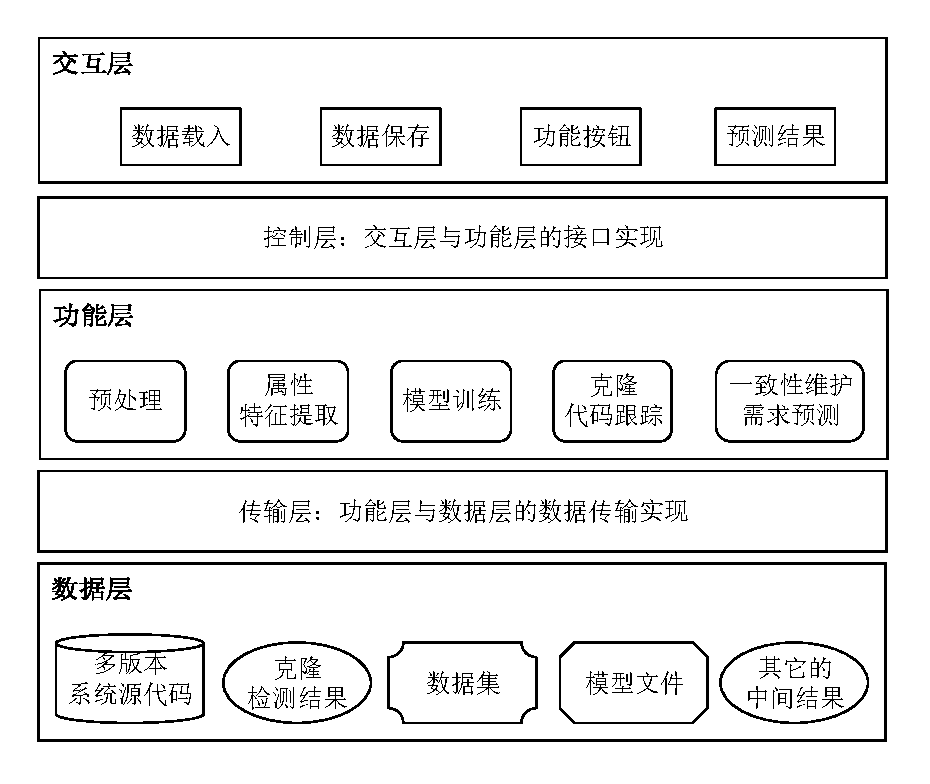
\includegraphics[width = 0.8\textwidth]{pluginframework.pdf}
\bicaption[pluginframework]{}{克隆一致性维护需求预测插件的体系结构}{Fig.$\!$}
{The framework for the plug-in of clone consistency-requirement prediction}
\vspace{-1em}
\end{figure}

\BiSubsection{克隆一致性维护需求预测插件的功能模块设计}
{The Design for Plug-in Function Modules of Clone Consistency Prediction}

本文的克隆代码一致性维护需求预测插件主要包括五个模块:预处理模块、属性提取模块、模型训练模块、克隆跟踪模块和预测模块。插件的模块设计如图~\ref{pluginmodule}~所示。预处理模块构建克隆家系并识别克隆演化模式,帮助程序开发人员收集系统中的克隆实例。属性提取模块实现对克隆实例的表示,提取不同的属性组表示相对应的克隆实例。预测模块可以根据不同用户需求,通过调用WEKA中的机器学习算法,构建和训练克隆一致性维护需求的预测器。克隆跟踪模块可以跟踪系统中的克隆代码产生和变化。预测模块可以根据克隆跟踪的过程,对新产生的克隆代码和克隆代码的变化进行一致性维护需求预测。

\begin{figure}[htbp]
\centering
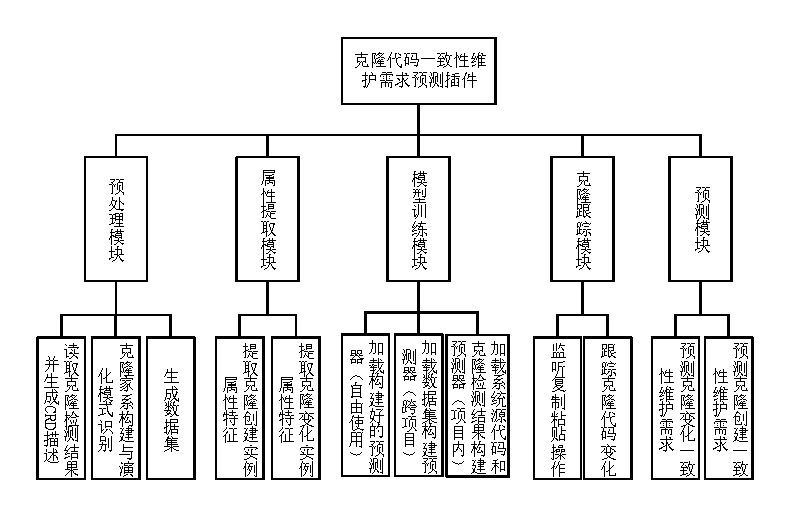
\includegraphics[width = 0.8\textwidth]{pluginmodule.pdf}
\bicaption[pluginmodule]{}{克隆一致性维护插件的功能模块}{Fig.$\!$}
{The modules for clone consistency-requirement prediction}
\vspace{-1em}
\end{figure}

(1)预处理模块

预处理模块通过识别克隆检测工具的检测结果,并构建克隆家系和识别克隆演化模式,从而收集并生成相应系统的克隆实例。首先,需要人工的使用克克隆检测工具检测系统中的所有的克隆代码,并将检测结果作为插件的输入,本文中使用的克隆检测工具是NiCad 。对于软件系统的每一个版本,克隆代码将会被组成克隆组的形式,并使用文件名、起始行号表示所有的克隆代码,即“{\tt file\_name}”、“{\tt start\_line}”和“{\tt end \_line}”。然后,使用CRD重新描述克隆代码并重新组织为新的数据结构,从而方便构建克隆家系。然后,本插件将基于CRD对所有版本中的克隆代码,构建构建系统的克隆家系,并识别克隆演化模式。方法参加本文克隆家系构建和模式识别部分。最后,根据所构建的克隆家系和识别的演化模式,可以方便的生成相应系统的克隆创建和变化实例,从而生成其相应的数据集。值得注意的是,完整的数据集需通过调用属性提取模块生成具体的属性特征。

(2) 属性提取模块

属性提取模块可以提取克隆实例的属性特征,将不同的克隆代码实例抽象成相应的属性值。对克隆创建实例,提取代码属性表示被复制的克隆代码,提取上下文属性表示被粘贴的克隆代码。对克隆变化实例,从克隆组的角度提取代码属性、上下文属性、演化属性和相对应的克隆变化情况。首先,对代码属性和上下文属性的提取,可以使用抽象语法树(Abstract Syntactic Tree,AST)对程序源代码进行解析并提取。对每一个克隆代码以及克隆代码所在文件,使用Eclipse AST中的 ASTParser类将克隆片段所在源代码解析成AST\footnote{抽象语法树可参见:http://www.eclipse.org/articles/Article-JavaCodeManipulation\_AST/}。通过遍历语法树访问相应关键节点,根据本文描述的属性值计算克隆实例的代码属性和上下文属性。然后,对于演化属性的提取,可以取通过遍历该克隆实例的克隆家系,根据对其属性的描述计算相应演化属性。

(3)模型训练模块

模型训练模块根据用户的请求,调用WEKA构建和训练机器学习模型。为灵活的使用本文方法,本文提供三种构建和训练预测模型的方式:

(a)项目内模型训练,该方式用项目自身的历史数据来训练预测模型。在这种情况下,本文的插件首先调用预处理模块,构建项目本身所有克隆家系和收集项目中的所有克隆实例。然后调用属性提取模块,将提取收集到的克隆实例的属性值,并生成训练集。最后,使用该训练集建立和训练机器学习模型,并将训练好的模型应用于克隆代码的一致性维护需求预测中。

(b)跨项目模型训练,该方式使用其它项目数据作为训练集来训练预测模型。在软件开发初期,由于演化时间较短导致其历史的克隆实例较少,不足以较好的训练所需要的模型。因此,需要使用其它项目的历史数据作为训练集。首先,用户指定相应的训练系统,并导入相应的输入数据。然后,通过调用预处理和属性特征提取模块生成所需的训练集。最后,使用训练集训练跨项目的预测模型,并将其应用于当前测试系统的一致性维护需求预测中。需要注意的是,随着时间的推移,当项目自身可以收集到足够的数据时,本文建议开发人员重新使用项目自身的数据训练机器学习模型,从而达到较好的预测效果。

(c)加载已有训练模型,该方式直接加载已经训练好的机器学习模型。由于机器学习模型的构建和训练往往需要大量的时间,开发人员不应该也不需要在每次开发时都训练机器学习模型。因此,在实际的开发过程中,模型的训练和开发时的预测可以分开进行。首先通过(a)和(b)两种方式进行模型的训练,然后使用(c)加载训练好的模型文件,最后进行克隆代码一致性维护需求预测。

(4)克隆代码跟踪模块

在软件开发过程中预测克隆代码的一致性需求维护,还需要实时的捕获软件中产生的克隆实例,即跟踪克隆实例的产生(克隆创建实例和克隆变化实例)。

首先,该模块可以跟踪开发人员的复制和粘贴操作。研究表明,软件中的克隆代码主要是由于复制和粘贴操作导致,即克隆创建实例产生的直接原因是程序开发人员的复制和粘贴操作。因此,监测复制和粘贴操作即可跟踪克隆创建实例的产生。但是,在实际的软件开发过程中,大部分的复制和粘贴操作是对一些具体的变量进行的,这些操作不会导致克隆代码。因此,本文对复制粘贴操作进行了筛选,认定复制和粘贴的代码行数最少为5行的操作,才是会导致克隆代码的复制和粘贴操作。

然后,该模块还可以跟踪系统中克隆代码的变化。对克隆代码跟踪的功能有两种实现的策略,一是根据CRD跟踪演化的克隆代码代码,而是通过eclipse开发平台所提供的文档内片段位置更新功能(位置更新器)实现。对于第一种方式,克隆代码的CRD中存储了其上下文信息,通过比较开发人员当前修改的代码片段是否和系统中的克隆代码区域重合,认定是否对克隆代码片段进行了修改。对于第二种方式,对于一个打开的文档,先确定该文档内是否含有克隆代码,如果含有克隆代码,则需要对其包含的克隆代码进行跟踪。位置跟踪器通过克隆代码片段的首字符在文档中的偏移量和片段长度来表示要跟踪的范围。将要跟踪的代码片段位置和跟踪其位置的更新器通过更新器种类绑定在一起,便可实现克隆片段的位置跟踪。然后,通过判断该克隆代码片段是否被修改(与上一版本比较),识别克隆代码的变化。

(5)预测模块

当监测到具体的克隆实例产生时,调用已经训练好的机器学习模型进行预测。软件开发过程中,监测到克隆实例产生时,调用属性提取模块提取本次实例的属性,并使用训练好的一致性模型预测其一致性维护需求。根据预测结果通知程序开发人员采取相应措施。值得注意的是,在实际预测时,克隆变化实例预测需要项目的历史版本源代码,因为历史属性中包含克隆变化实例的历史变化过程。为了轻量化预测过程,程序开发人员可以将当前版本中所有的克隆组的演化属性均提取出来。当克隆变化实例产生时,直接使用其作为属性,从而避免属性提取的时间。

\BiSubsection{克隆一致性维护需求预测插件的实现}
{The Implementation for Plug-in of Clone Consistency Prediction}

本文基于eclipse实现了克隆一致性维护需求预测插件。eclipse 是一个基于JAVA语言的开源集成开发环境,具有良好的可扩展性和跨平台性。eclipse是一个具有极小内核的开发平台,其所有功能都以插件的形式添加到此内核上。同时,eclipse具有极为友好的插件开发环境,用户可以根据自身需要开发所需的功能,并以插件的形式发布在eclipse平台上。因此,本文也选择ecilpse实现克隆代码的一致性维护需求预测插件。

同时,本文设计的插件需要对不同的机器学习模型进行训练,并对在软件开发过程进行一致性维护需求预测。为了实现此功能,本插件也集成了WEKA的软件开发包。WEKA是一个JAVA语言实现的数据挖掘和机器学习开源工具,提供了丰富的接口帮助程序开发人员调用相关的机器学习方法,从而极为灵活的进行模型的训练和预测\footnote{使用WEKA可参见:http://weka.wikispaces.com/。}。

本文所设计的插件运行截图如图~\ref{pluginview1}~所示。由图中看出,本章实现的插件会在eclipse开发环境的菜单栏中,新增加一个新的菜单项“Clones”。该菜单具备克隆一致性维护需求预测的功能。
%因此,插件的安装方式,和普通的eclipse插件安装方式一样。一个简单的安装方法为:将插件(Myplugin.CloneControl.jar)复制到eclipse的主目录下的plugins文件夹中。然后重启eclipse,克隆一致性维护需求预测插件可以在eclipse的工作窗口中可见。

\begin{figure}[htbp]
\centering
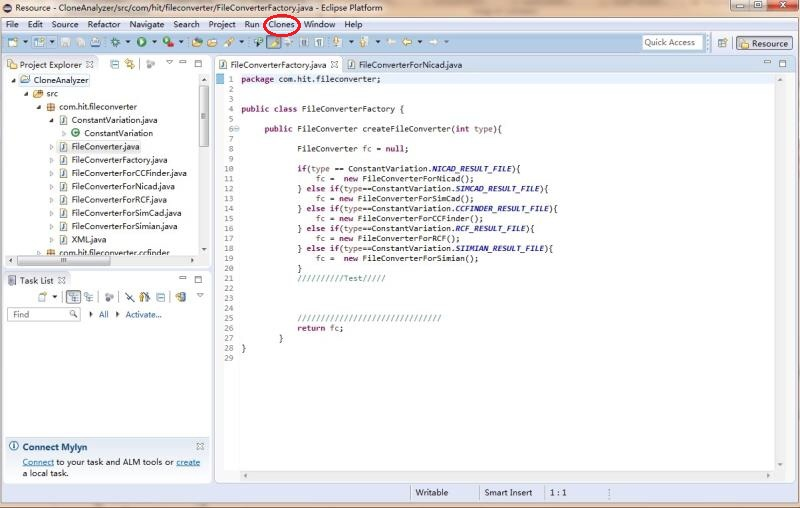
\includegraphics[width = 0.8\textwidth]{plugin1.jpg}
\bicaption[pluginview1]{}{插件安装完成后Eclipse界面}{Fig.$\!$}
{The screen-shot for eclipse with installed plug-in of clone consistency prediction}
\vspace{-1em}
\end{figure}

在使用本文所设计的一致性维护需求预测插件时,需要提前加载已训练好的机器学习模型。为方便用户使用,本章插件提供三种方式加载预测模型:(1)加载系统源代码及克隆检测工具的检测结果构建预测模型(项目内);(2)加载已有软件历史版本特征向量训练预测模型(跨项目)。(3)加载已有预测模型。加载所需功能截图如图~\ref{pluginview2}~所示。%其中Show Clones 菜单项是显示当前通过复制粘贴形成的克隆代码、已经被程序开发人员修改的克隆代码。

\begin{figure}[htbp]
\centering
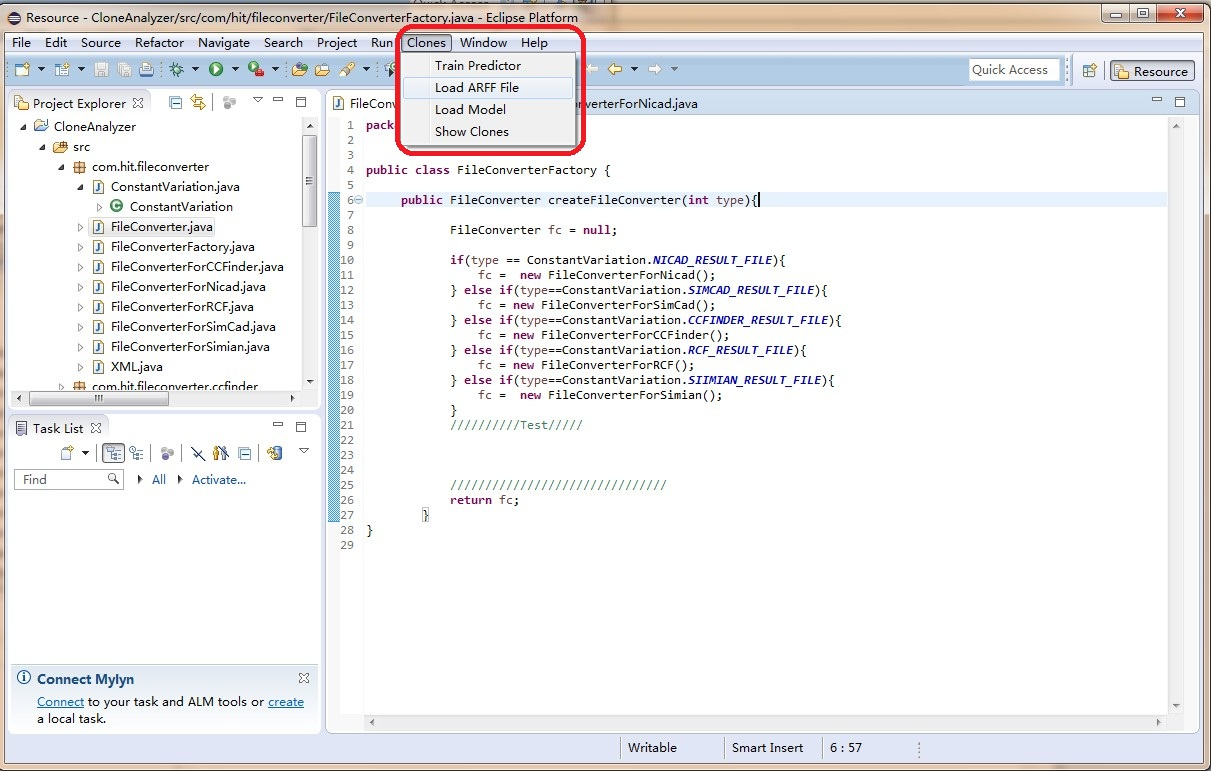
\includegraphics[width = 0.8\textwidth]{plugin2.jpg}
\bicaption[pluginview2]{}{插件加载预测模型的截图}{Fig.$\!$}
{The screen-shot for loading the models of clone consistency prediction}
\vspace{-1em}
\end{figure}

成功加载预测模型后,该插件便可以预测克隆代码的一致性维护需求。通过监听开发过程中的克隆创建和变化实例,并预测克隆代码的一致性维护需求。图中~\ref{pluginview3}~是一个会导致额外维护代价的克隆创建操作的警告示例。如图所示,本插件会警告软件开发人员,其操作会引发额外的维护代价。根据预测结果,开发人员可以采取拒绝此复制粘贴操作,以避免在其未来演化过程中的克隆代码的额外维护代价。

\begin{figure}[htbp]
\centering
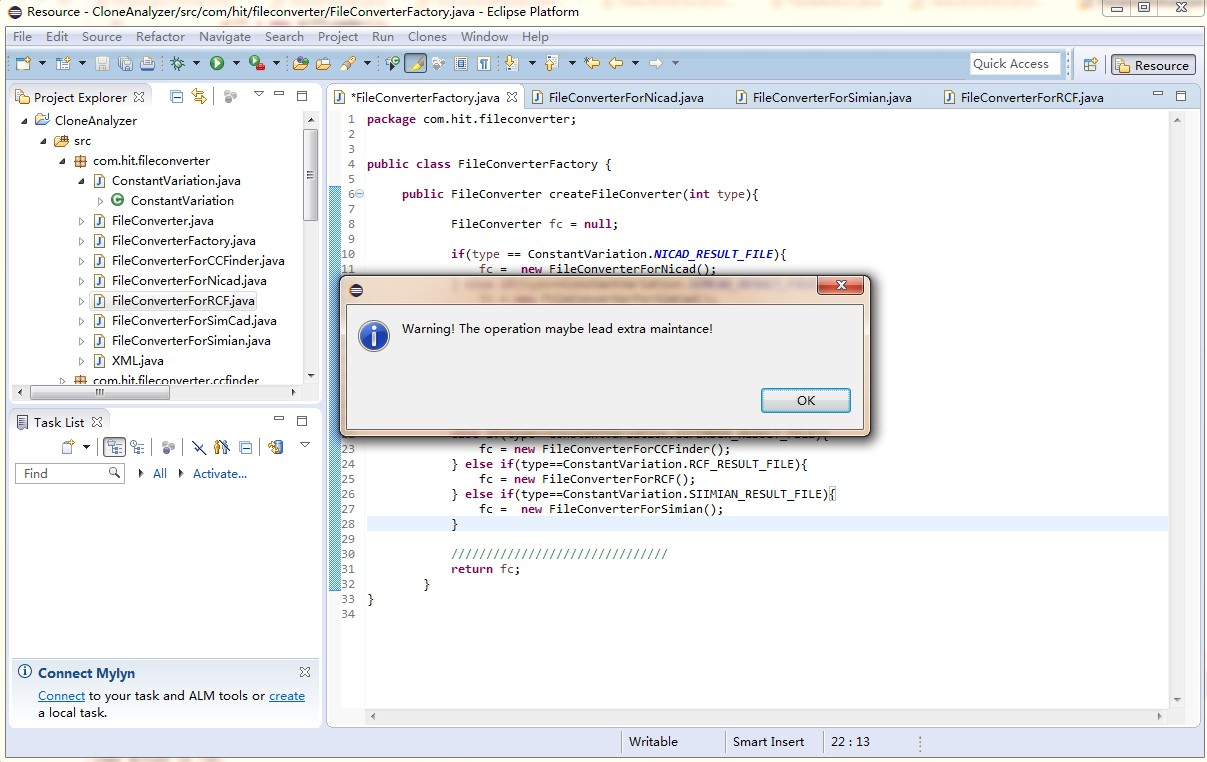
\includegraphics[width = 0.8\textwidth]{plugin3.jpg}
\bicaption[pluginview3]{}{需要一致性维护的预测结果示例}{Fig.$\!$}
{The screen-shot for a prediction example that meeting consistency}
\vspace{-1em}
\end{figure}

%%%%%当通过软件源代码和克隆检测结果加载预测模型时,需要对克隆检测结果进行处理,提取表示克隆代码的特征,并生成特征文件作为训练集,训练预测模型。该部分最初设计成一个独立的Application, 最后将其打成Jar 包嵌入到Eclipse 开发环境中。
%%%%%本节主要介绍最初的独立的Application, 以说明该模块功能。该Application的界面进行简单处理,运行界面如图2-1所示。

%%%% 
%%%% \begin{figure}[htbp]
%%%%\centering
%%%%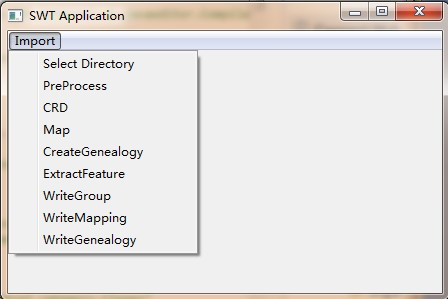
\includegraphics[width = 0.4\textwidth]{plugin4.jpg}
%%%%\bicaption[pluginview3]{}{插件安装完成后Eclipse界面}{Fig.$\!$}
%%%%{The screen-shot of eclipse after install our plug-in}
%%%%\vspace{-1em}
%%%%\end{figure}
%%%% 
%%%%图2-1 Application运行界面
%%%%主要包括五个功能,构建克隆区域描述符(CRD),构建相邻版本间克隆代码的映射关系(Map),生成克隆家系(CreateGenealogy),提取训练需要的各种特征形成特征文件(ExtractFeature),以及克隆表示的测试(WriteGroup,WriteMapping,WriteGenealogy),分别单击每一项,完成相应功能。Select Directory 项是加载软件系统源代码路径和克隆检测结果路径,其中源代码路径给到包括各种历史版本源代码的文件夹路径,如SubjectSys\_jEdit 文件夹下存放jEdit 系统的多版本源代码路径,则源代码路径给到SubjectSys\_jEdit 文件夹。克隆检测结果路径给到检测结果的上层路径,例如Nicad 的检测结果是按克隆粒度存放的,例如jEdit 系统使用Nicad 按块进行检测的结果存放形式是jEdit 文件夹下有block 文件夹,block 文件夹才存放克隆检测结果,因此路径给到jEdit文件夹 而不是block 文件夹。PreProcess 项是调用所有功能,从构建克隆代码的CRD 信息到生成特征文件。因为当系统中克隆代码过多时,调用PreProcess 结果较慢,因此将每个功能单独出来方便测试,观察结果

\BiSection{本章小结}
{Summary of this Chapter}

在软件开发过程中,克隆代码的一致性变化会增加软件维护的代价。然而,软件开发初期由于克隆实例较少,无法训练机器学习模型进行一致性预测。因此,本章在第3章和第4章研究的基础上,统一了克隆创建和变化的一致性维护需求定义,并结合软件开发过程,对跨项目的克隆代码一致性维护需求预测进行研究。在四个开源系统上进行了跨项目实验,从三个不同的角度回答了本章所提出的研究问题。跨项目的预测实验结果表明:在软件开发初期阶段,可以使用跨项目的训练数据训练机器学习模型,并应用于其它系统的克隆一致性需求预测中。同时,由于样本的不平衡性,不推荐使用SVM模型进行跨项目预测。训练集的规模会对跨项目的预测能力产生影响,建议增大训练集的规模,但是仍然无法弥补项目之间的差异性。最后,本章设计和开发了一个克隆代码一致性预测插件,可以帮助程序开发人员在实际的开发过程中预测克隆代码的一致性,帮助提高软件的可维护性和软件质量。